\documentclass{beamer}

% Beamer style
%\usetheme[secheader]{Madrid}
\usetheme{CambridgeUS}
\usecolortheme[rgb={0.65,0.15,0.25}]{structure}
%\usefonttheme[onlymath]{serif}
\beamertemplatenavigationsymbolsempty
%\AtBeginSubsection

% Packages
%\usepackage[french]{babel}
\usepackage[latin1]{inputenc}
\usepackage{color}
%\usepackage{dsfont, stmaryrd}
\usepackage{amsmath, amsfonts, amssymb}
%\usepackage{stmaryrd}
\usepackage{epsfig}
\usepackage{../../../../LATEX/astats}
%\usepackage[all]{xy}
\usepackage{graphicx}

% Commands
\definecolor{darkred}{rgb}{0.65,0.15,0.25}
\definecolor{darkgreen}{rgb}{0,0.4,0}
%\newcommand{\emphase}[1]{\textcolor{darkred}{#1}}
\newcommand{\emphase}[1]{{#1}}
\newcommand{\paragraph}[1]{\textcolor{darkred}{#1}}
\newcommand{\refer}[1]{\textcolor{blue}{\sl \cite{#1}}}
\newcommand{\Refer}[1]{\textcolor{blue}{\sl #1}}
\newcommand{\newblock}{}

% Symbols
\newcommand{\Abf}{{\bf A}}
\newcommand{\Beta}{\text{B}}
\newcommand{\betabf}{\text{\mathversion{bold}{$\beta$}}}
\newcommand{\Bcal}{\mathcal{B}}
\newcommand{\BIC}{\text{BIC}}
\newcommand{\dd}{\text{d}}
\newcommand{\Cbf}{{\bf C}}
\newcommand{\dbf}{{\bf d}}
\newcommand{\Dcal}{\mathcal{D}}
\newcommand{\Esp}{\mathbb{E}}
\newcommand{\Ebf}{{\bf E}}
\newcommand{\Ecal}{\mathcal{E}}
\newcommand{\Gcal}{\mathcal{G}}
\newcommand{\Gam}{\mathcal{G}\text{am}}
\newcommand{\Ibb}{\mathbb{I}}
\newcommand{\Ibf}{{\bf I}}
\newcommand{\ICL}{\text{ICL}}
\newcommand{\Cov}{\mathbb{C}\text{ov}}
\newcommand{\Corr}{\mathbb{C}\text{orr}}
\newcommand{\Var}{\mathbb{V}}
\newcommand{\Vsf}{\mathsf{V}}
\newcommand{\pen}{\text{pen}}
\newcommand{\Fcal}{\mathcal{F}}
\newcommand{\Hbf}{{\bf H}}
\newcommand{\Hcal}{\mathcal{H}}
\newcommand{\Jcal}{\mathcal{J}}
\newcommand{\Kbf}{{\bf K}}
\newcommand{\Lcal}{\mathcal{L}}
\newcommand{\Lbf}{{\bf L}}
\newcommand{\Mcal}{\mathcal{M}}
\newcommand{\mbf}{{\bf m}}
\newcommand{\mum}{\mu(\mbf)}
\newcommand{\Ncal}{\mathcal{N}}
\newcommand{\Nbf}{{\bf N}}
\newcommand{\Nm}{N(\mbf)}
\newcommand{\Ocal}{\mathcal{O}}
\newcommand{\Obf}{{\bf 0}}
\newcommand{\Omegas}{\underset{s}{\Omega}}
\newcommand{\Pbf}{{\bf P}}
\newcommand{\Pcal}{\mathcal{P}}
\newcommand{\Qcal}{\mathcal{Q}}
\newcommand{\Rbb}{\mathbb{R}}
\newcommand{\Rcal}{\mathcal{R}}
\newcommand{\sbf}{{\bf s}}
\newcommand{\Sbf}{{\bf S}}
\newcommand{\Scal}{\mathcal{S}}
\newcommand{\Ucal}{\mathcal{U}}
\newcommand{\Vcal}{\mathcal{V}}
\newcommand{\Tbf}{{\bf T}}
\newcommand{\ubf}{{\bf u}}
\newcommand{\Ubf}{{\bf U}}
\newcommand{\Wbf}{{\bf W}}
\newcommand{\xbf}{{\bf x}}
\newcommand{\Xbf}{{\bf X}}
\newcommand{\Ybf}{{\bf Y}}
\newcommand{\Zbf}{{\bf Z}}
\newcommand{\pibf}{\text{\mathversion{bold}{$\pi$}}}
\newcommand{\Sigmabf}{\text{\mathversion{bold}{$\Sigma$}}}
\newcommand{\gammabf}{\text{\mathversion{bold}{$\gamma$}}}
\newcommand{\mubf}{\text{\mathversion{bold}{$\mu$}}}
\newcommand{\nubf}{\text{\mathversion{bold}{$\nu$}}}
\newcommand{\Thetabf}{\text{\mathversion{bold}{$\Theta$}}}
\newcommand{\thetabf}{\text{\mathversion{bold}{$\theta$}}}
\newcommand{\BP}{\text{BP}}
\newcommand{\EM}{\text{EM}}
\newcommand{\VEM}{\text{VEM}}
\newcommand{\VBEM}{\text{VB}}
\newcommand{\cst}{\text{cst}}
\newcommand{\obs}{\text{obs}}
\newcommand{\ra}{\emphase{$\rightarrow$~}}
\newcommand{\QZ}{Q_{\Zbf}}
\newcommand{\Qt}{Q_{\thetabf}}

% Directory
\newcommand{\fighd}{../Figures}
\newcommand{\figSimHMM}{../FIGURES/CGH-HMM-sim/CGHsim-9}


%====================================================================
\title[Change-point and chromosomal alterations]{Change-point detection 
  for the analysis of chromoso0mal alterations}

\author[S. Robin]{S. Robin}

\institute[AgroParisTech / INRA]{UMR 518 AgroParisTech / INRA Applied
  MAth \& Comput. Sc.\\
  \bigskip
  \begin{tabular}{ccccc}
    
\epsfig{file=../FIGURES/LogoINRA-Couleur.ps,
    width=2.5cm} & 
    \hspace{.5cm} &
    
\epsfig{file=../FIGURES/logagroptechsolo.eps,
    width=3.75cm} & 
    \hspace{.5cm} &
    
\epsfig{file=../FIGURES/logo-ssb.eps,
    width=2.5cm} \\ 
  \end{tabular} \\
  \bigskip
  }

  \date[Biogemma]{S�minaire Biogemma, April 2013}

%====================================================================

%====================================================================
%====================================================================
\begin{document}
%====================================================================
%====================================================================

%====================================================================
\frame{\titlepage
  }

%====================================================================
\frame{\frametitle{Outline} 
  \tableofcontents
  }

%====================================================================
%====================================================================
\section{Segmentation: The basic problem}
\frame{\frametitle{Segmentation: The basic problem}}
% ====================================================================
\frame{ \frametitle{Copy number variations in cancer cells} 
  Genomic alterations are associated with (responsible for?) various
  types of cancers.
  
  \begin{tabular}{cc}
    \onslide+<1->{Normal cell} & \onslide+<2->{Tumor cell} \\
    \onslide+<1->{
      \epsfig{file =
        \fighd/KaryotypeCancer-PH.ps, clip=,
        bbllx=325, bblly=676, bburx=468, bbury=780, scale=.9} 
    }
    &
    \onslide+<2->{
      \epsfig{file =
        \fighd/KaryotypeCancer-PH.ps, clip=,
        bbllx=127, bblly=676, bburx=319, bbury=780, scale=.9} 
    }
  \end{tabular}
  
  \onslide+<2->{
    Source: \refer{Hup08}. 
  }
}

%====================================================================
\frame{\frametitle{Array CGH technology: Principle}
  
\epsfig{file = ../FIGURES/principe_CGH.eps, clip=,
  bbllx=0, bblly=41, bburx=700, bbury=478, width=.9\textwidth}
}

%====================================================================
\frame{\frametitle{An example}

  \hspace{-.5cm}
  \begin{tabular}{ccccc}
    \multicolumn{3}{c}{Zoom on CGH profile} & \quad & Karyotype \\
    chrom. 1 & \quad & chrom. 17 \\
    \begin{tabular}{c}
      % \epsfig{file = ../FIGURES/Karyotype-CGH-PH.ps, clip=,
      % bbllx=80, bblly=617, bburx=150, bbury=763, scale=2}
      \epsfig{file = ../FIGURES/Karyotype-CGH-PH.ps, clip=,
        bbllx=80, bblly=617, bburx=150, bbury=700, height=.5\textheight}
    \end{tabular}
    & &
    \begin{tabular}{c}
      % \epsfig{file = ../FIGURES/Karyotype-CGH-PH.ps, clip=,
      % bbllx=270, bblly=617, bburx=300, bbury=763, scale=2}
      \epsfig{file = ../FIGURES/Karyotype-CGH-PH.ps, clip=,
        bbllx=270, bblly=617, bburx=300, bbury=700, height=.5\textheight}
    \end{tabular}
    & &
    \begin{tabular}{c}
      \epsfig{file = ../FIGURES/Karyotype-CGH-PH.ps, clip=,
        bbllx=364, bblly=617, bburx=485, bbury=763, height=.5\textheight}
    \end{tabular}
  \end{tabular}

  \bigskip
  (\refer{Hup08})

}

%====================================================================
\frame{\frametitle{Segmentation: The basic problem}

  %\vspace{-0.5cm}
  \begin{tabular}{cc}
    \begin{tabular}{p{.5\textwidth}}
      \onslide+<1->{
        \paragraph{Data at hand:} for a given individual
        \begin{itemize}
        \item a sequence of \emphase{known positions} along the
          \emphase{reference genome}, labeled as
          $$
          t = 1, 2, \dots, n
          $$
        \item a signal measured \emphase{at each position}
          $$
          Y_t = \text{signal at position $t$}
          $$
        \end{itemize}
        }
    \end{tabular}
    &
    \begin{tabular}{p{.5\textwidth}}
      \hspace{-1cm}
      \begin{overprint}
        \onslide<2-3>
        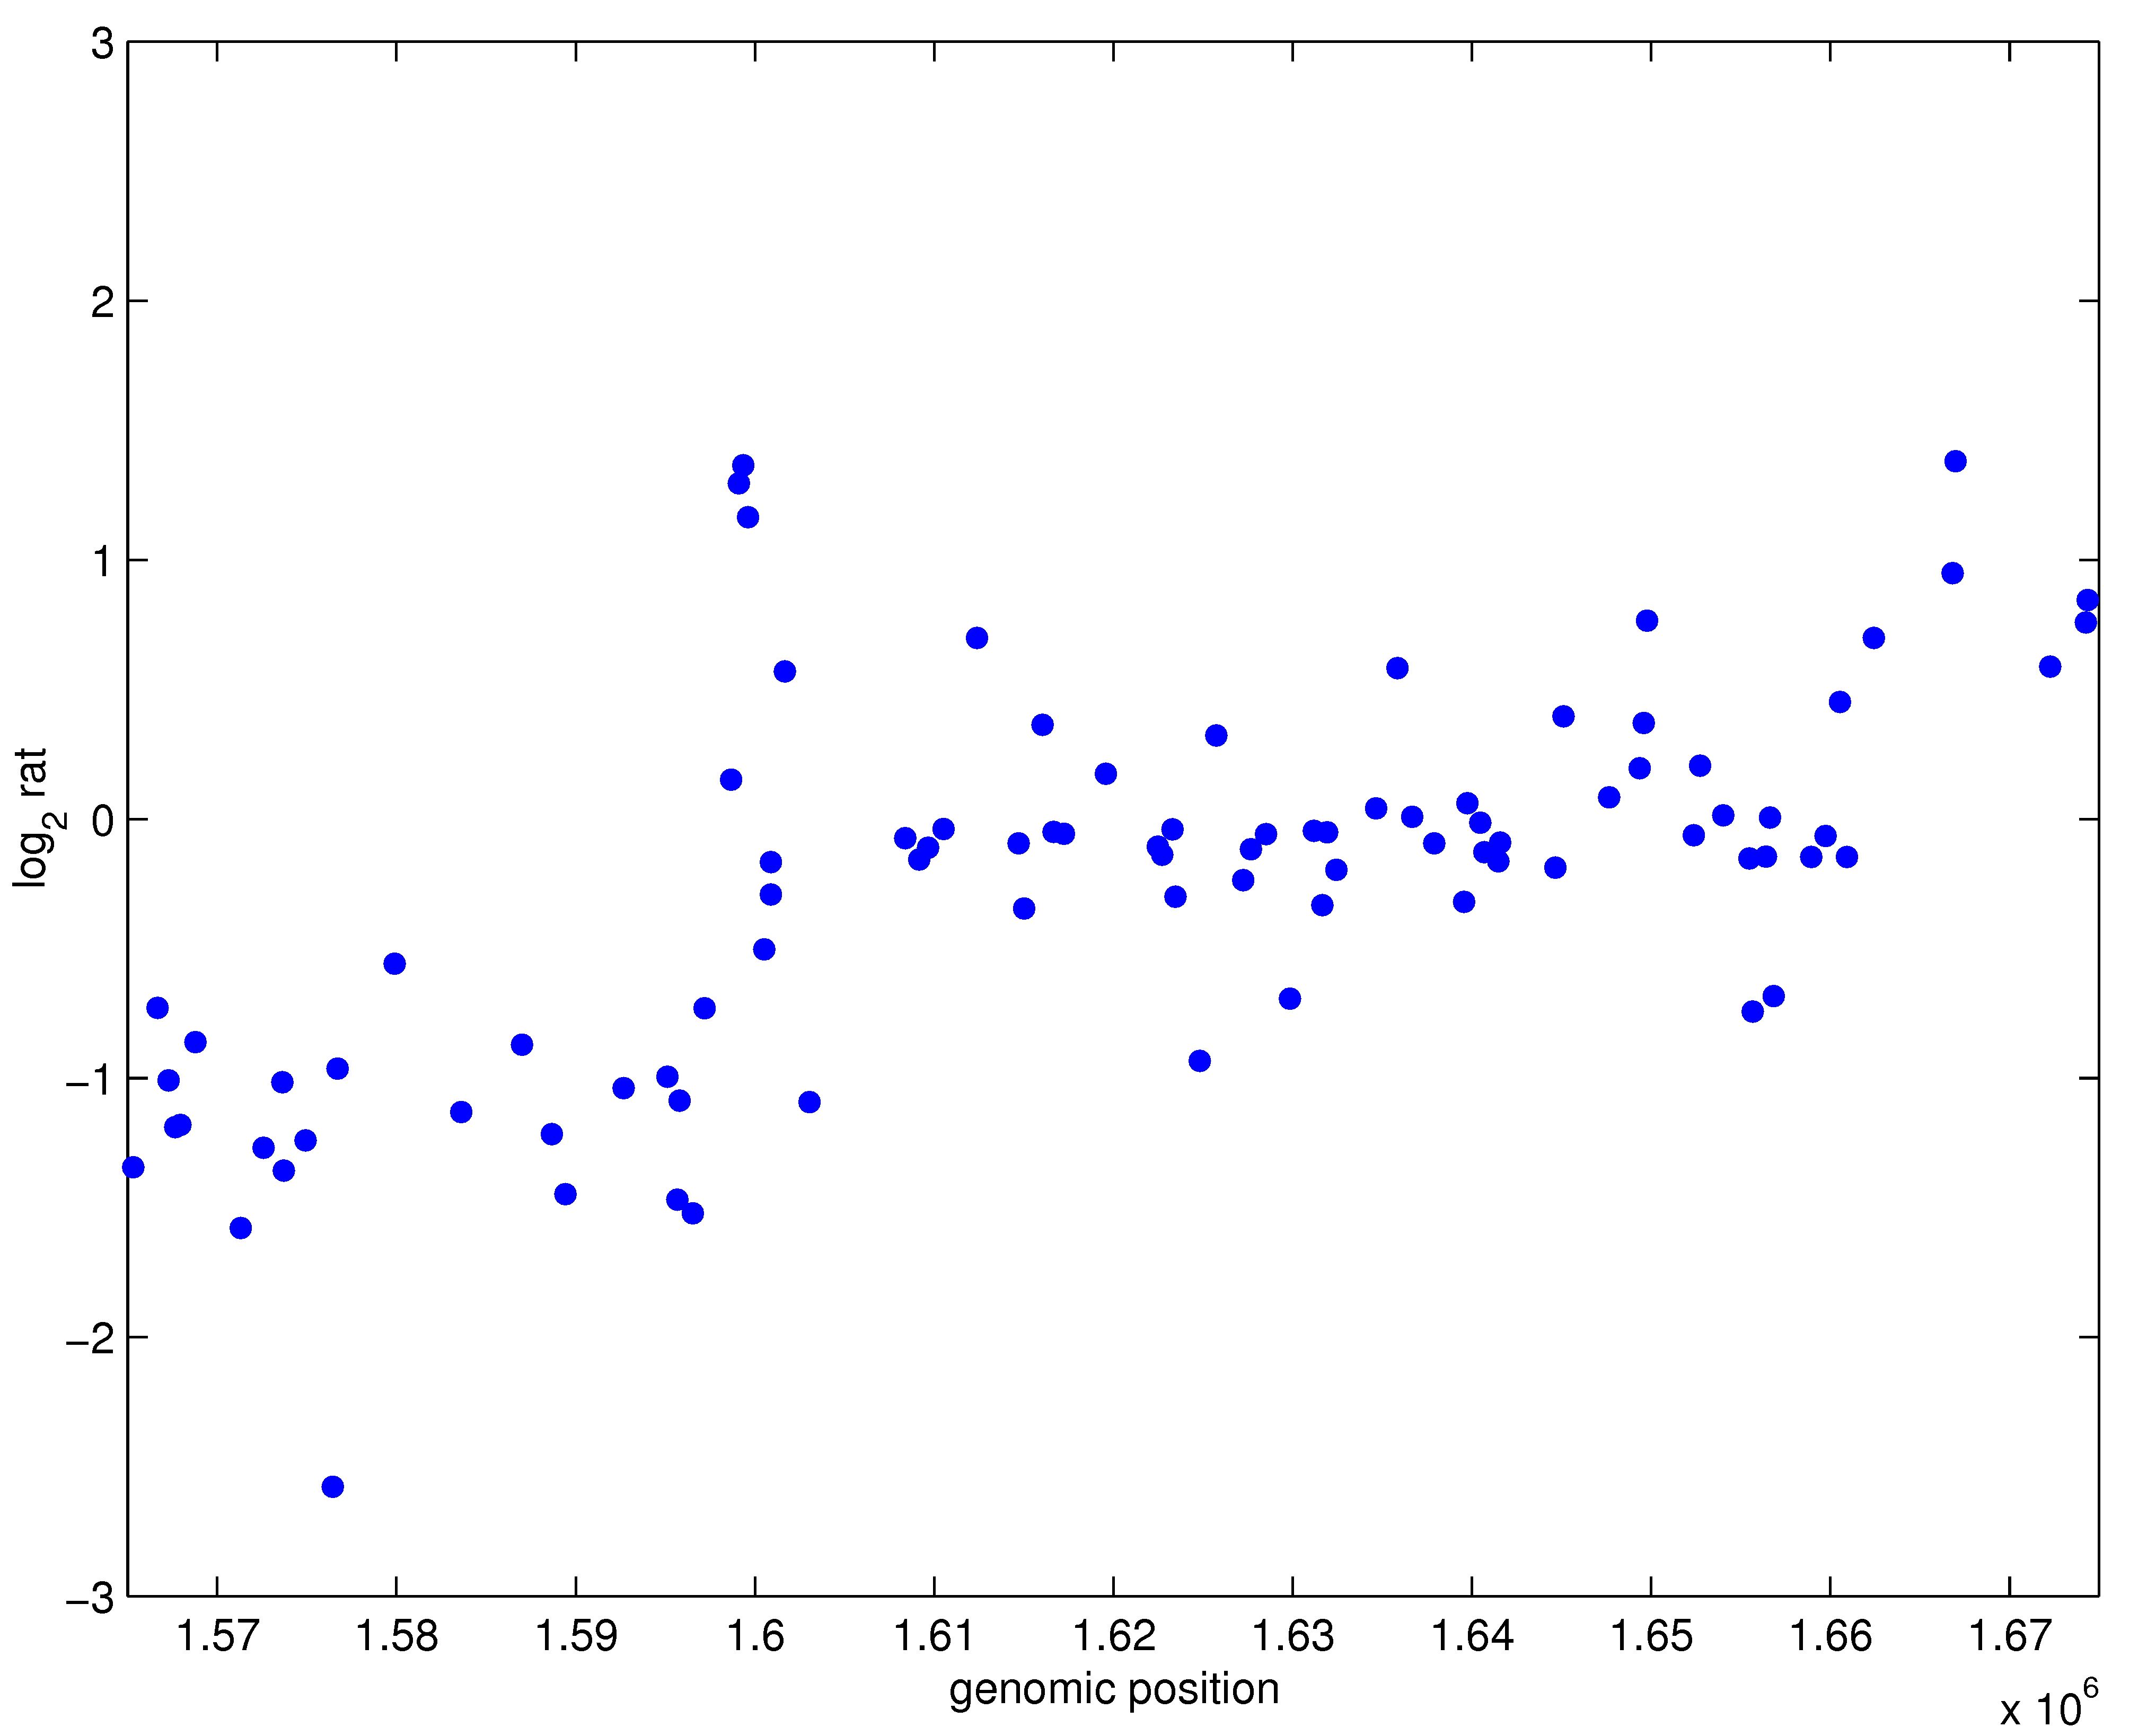
\epsfig{file = ../FIGURES/raw_profile_example.eps, clip=,
          width=.45\textwidth, height=.5\textheight}  
        \onslide<4>
        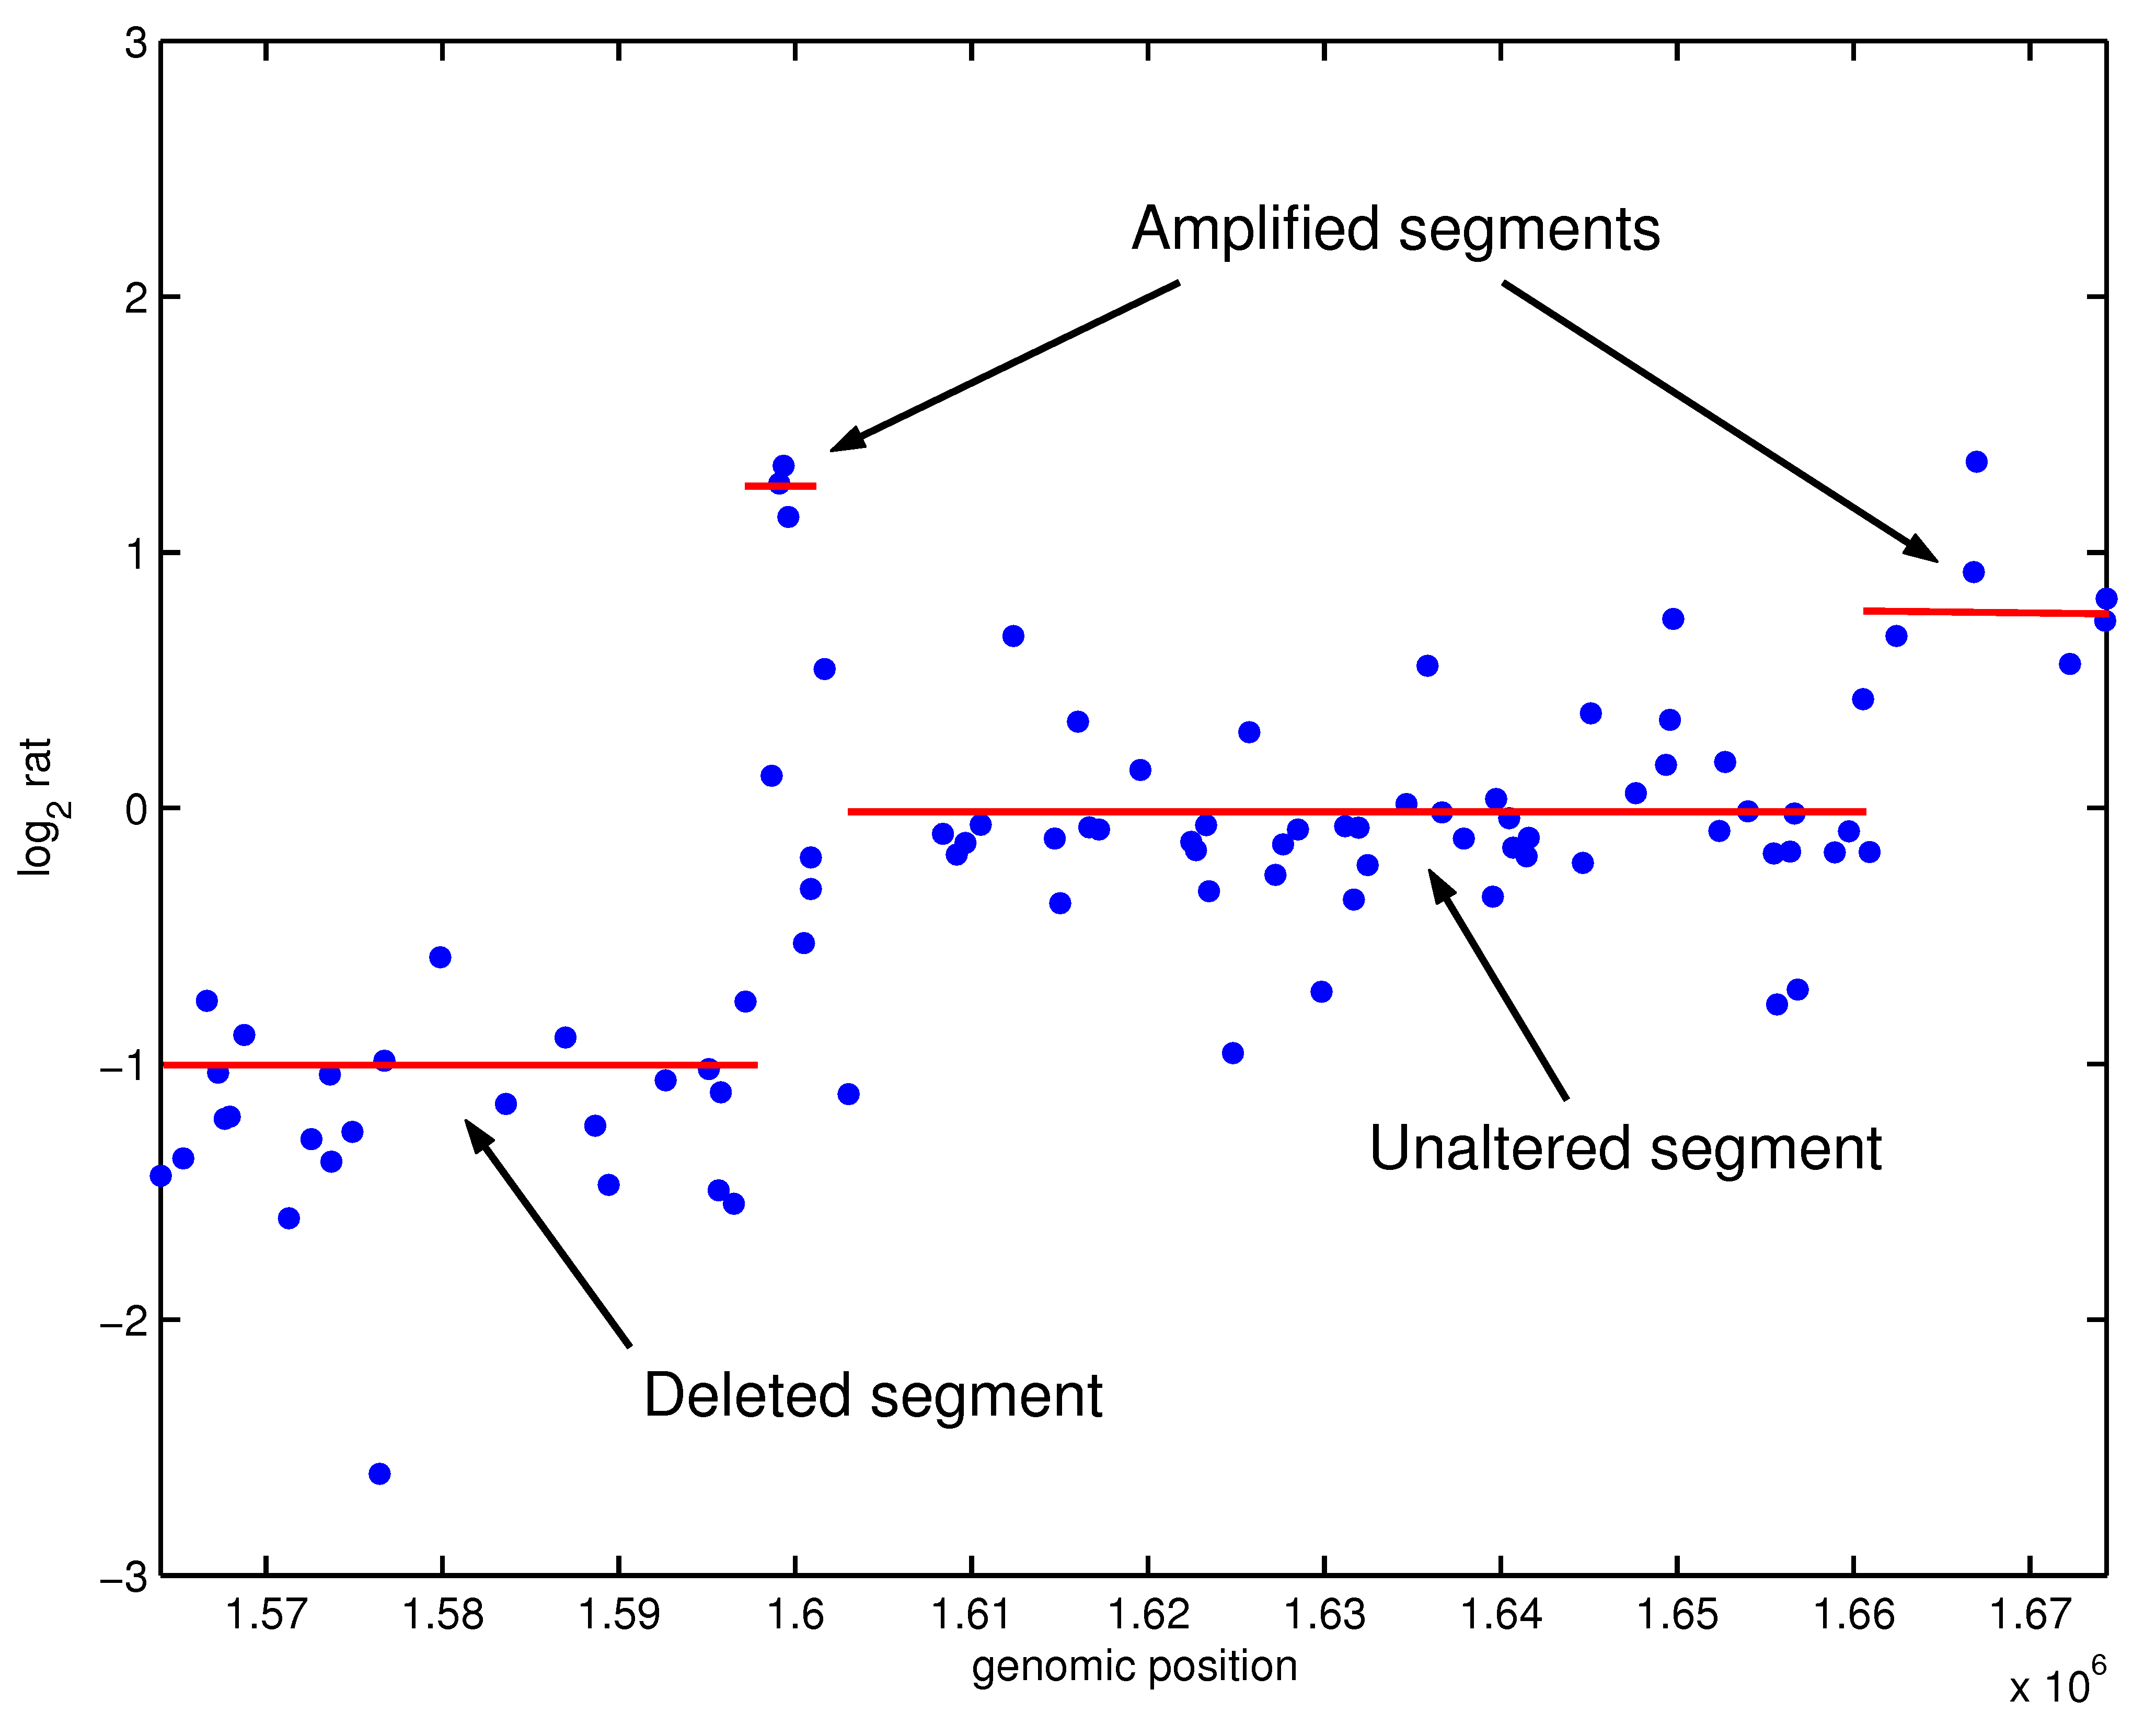
\epsfig{file = ../FIGURES/profile_example.eps, clip=,
          %bbllx=60, bblly=196, bburx=543, bbury=586}
          width=.45\textwidth, height=.5\textheight}  
      \end{overprint}
    \end{tabular}
  \end{tabular} \\
  \onslide+<3->{
    \begin{eqnarray*}
      Y_t & \propto & f(\text{\emphase{relative copy number} at position }t) \\
      & = & \text{log-fluorescence, sum of the two allele signals for a given
        SNP, etc.}
    \end{eqnarray*}
    }
  }

%%====================================================================
%%====================================================================
%\section{Segmentation model for one profile}
%\frame{\frametitle{Segmentation model for one profile}}
%%====================================================================

%====================================================================
\subsection*{Statistical model}
%====================================================================
\frame{\frametitle{A model, what for?}
  
  \begin{itemize}
  \item To \emphase{translate biological questions into mathematical equations} and quantities;
  \item To make \emphase{all hypotheses explicit};
  \item To set the inference of interesting parameters in a
    \emphase{global framework}, possibly accounting for other effects
    (covariates);
  \item To \emphase{motivate all calculations} and data processing to
    come.
  \end{itemize}
  
  \bigskip\pause
  \centerline{\emphase{The model is the place where biologist's and
      mathematician's minds meet.}}
  
  \bigskip\bigskip\pause
  \paragraph{Model-based approach.}
  \begin{itemize}
  \item Define a model that describes the biological process as well
    as possible;
  \item Make sure that it can be handled in terms of mathematics /
    statistics;
  \item Derive an (efficient and statistically valid) inference
    procedure.
  \end{itemize}
}

%====================================================================
\subsection*{Two models for the same question}
%====================================================================
\frame{\frametitle{Two models for the same question} 
  
  Change point detection can be tackled in various ways. Among model-based approaches, the most popular two are
  \begin{enumerate}
   \item segmentation models;
   \item hidden Markov models.
  \end{enumerate}

   \bigskip\pause
   Both approaches have pros and cons as they differ in terms of
   \begin{itemize}
    \item Models: underlying assumptions about the phenomenon at hand;
    \item Aim: segment classification (calling) or not; 
    \item Flexibility: what kind of dependency can we account for?
    \item Computational efficiency: linear ($\times$ ?) vs quadratic;
    \item Optimization guaranties: are we sure to get the 'optimal' segmentation?
    \item Statistical guaranties: what can be said about the precision of change point location? 
   \end{itemize}

 }

%====================================================================
\frame{\frametitle{Segmentation model for one series} 
  
  \begin{tabular}{cc}
    \hspace{-.5cm}
    \begin{tabular}{p{.5\textwidth}}
      \onslide+<2->{\paragraph{Statistical model.} 
        \begin{itemize}
        \item $\text{Signal} = f(\text{Position})$; \\}
        \onslide+<3->{
        \item Breakpoint positions: \\
          $\tau_1, \tau_2, ..., \tau_{K-1};$ \\}
        \onslide+<4->{
        \item Mean signal (relative copy number) within each interval: \\
          $\mu_1, \mu_2, ..., \mu_K$; \\}
        \onslide+<5->{
        \item Observed signal (log-ratio) at time $t=$ \\
          mean + i.i.d. noise $\Ncal(0, \sigma^2)$.
        \end{itemize}}
    \end{tabular}
    & 
    \hspace{-1cm}
    \begin{tabular}{c}
      \begin{overprint}
        \onslide<2>
        $\qquad \qquad \;\;\, Y_t =$ \\
        \epsfig{file=../FIGURES/FigSeg-Budapest-1.eps, clip=,
          angle=270, width=.5\textwidth} 
        \onslide<3>
        if $t \in \textcolor{blue}{I_k}, \quad Y_t =$ \\
        \epsfig{file=../FIGURES/FigSeg-Budapest-2.eps, clip=,
          angle=270, width=.5\textwidth} 
        \onslide<4>
        if $t \in \textcolor{blue}{I_k}, \quad Y_t = \textcolor{red}{\mu_k}$ \\
        \epsfig{file=../FIGURES/FigSeg-Budapest-3.eps, clip=,
          angle=270, width=.5\textwidth} 
        \onslide<5->
        if $t \in \textcolor{blue}{I_k}, \quad Y_t =
        \textcolor{red}{\mu_k} + E_t$ \\ 
        \epsfig{file=../FIGURES/FigSeg-Budapest-4.eps, clip=,
          angle=270, width=.5\textwidth} 
      \end{overprint}
    \end{tabular}
  \end{tabular}
  
%  \onslide+<6->{
%    \paragraph{Aim:}
%    Retrieve the 'true' number of segments \emphase{$K$},
%    change-points locations \emphase{$(\tau_k)$} and means
%    \emphase{$(\mu_k)$} ... within a reasonable time.
%  }
  
}

%====================================================================
\frame{\frametitle{Hidden Markov model for one series}

  \vspace{-0.5cm}
  \begin{tabular}{cc}
    \hspace{-.5cm}
    \begin{tabular}{p{.5\textwidth}}
    \onslide+<1->{\paragraph{Statistical model.} }
      \begin{itemize}
      \item \onslide+<1->{$t = 1..n$ probes (positions) are observed. \\~}
      \item \onslide+<2->{A (Markov) succession of \emphase{labels $Z_t$}
          ('loss', '\textcolor{red}{normal}',
          '\textcolor{darkgreen}{gain}') is associated with each probe. \\~}
      \item \onslide+<3->{The distribution of the \emphase{observed signal
          $Y_t$} depends on the label. \\~}
      \item \onslide+<4->{The labels are \emphase{hidden}.}
%      \item \onslide+<4->{We only observe the signal;}
%      \item \onslide+<5->{And we would like to retrieve the 'truth'.}
      \end{itemize}
    \end{tabular}
    &    \hspace{-1cm}
    \begin{tabular}{p{.5\textwidth}}
      \begin{overprint}
        \onslide<1>
          ~ \\ ~ \\
        \epsfig{file=\figSimHMM/SimHMM_n100_Q3.eps,
          width=0.4\textwidth, height=0.7\textheight, angle=270, clip=}
        \onslide<2>
        $\qquad \qquad (Z_t)\sim MC(\pi)$ \\ ~\\
        \epsfig{file=\figSimHMM/SimHMM_n100_Q3_Z.eps,
        width=0.4\textwidth, height=0.7\textheight, angle=270, clip=} 
        \onslide<3>
        $\qquad \qquad (Z_t)\sim MC(\pi)$ \\
        $\text{~~~~~if } Z_t=\textcolor{red}{k}, \quad Y_t = \textcolor{red}{\mu_k} + E_t$ \\
        \epsfig{file=\figSimHMM/SimHMM_n100_Q3_ZX.eps,
          width=0.4\textwidth, height=0.7\textheight, angle=270, clip=}         
        \onslide<4>
        $\qquad \qquad (Z_t)\sim MC(\pi)$ \\
        $\text{~~~~~if } Z_t=\textcolor{red}{k}, \quad Y_t = \textcolor{red}{\mu_k} + E_t$ \\
        \epsfig{file=\figSimHMM/SimHMM_n100_Q3_X.eps,
          width=0.4\textwidth, height=0.7\textheight, angle=270, clip=}
%        \onslide<5->
%        if $t \in \textcolor{blue}{I_k}, \quad Y_t =
%        \textcolor{red}{\mu_k} + E_t$ \\ 
%        \epsfig{file=../FIGURES/FigSeg-Budapest-4.eps, clip=,
%          angle=270, width=.5\textwidth} 
      \end{overprint}
    \end{tabular}
  \end{tabular} 
%  \\
%  \onslide+<6->{(Although we know we won't succeed.)}
  
}

%====================================================================
\frame{\frametitle{Parameters of the two models} 

  \vspace{-0.5cm}
  \begin{tabular}{p{.2\textwidth}cp{.3\textwidth}cp{.3\textwidth}}
    & & \paragraph{Segmentation} &  & \paragraph{HMM} \\ 
    \hline
    \\
    Dimension &  &$K =$ number of segments &  &$Q=$ number of labels \\ \pause
      \\
    Change-points parameters &  &change-point locations $\tau_1, ... \tau_{K-1}$ &  &transition probabilities $\pi(q, \ell)$ \\ \pause
      \\
    \vspace{.75cm} Distribution of the observed signal & &
    \multicolumn{3}{p{.7\textwidth}}{
    $$
    Y_t \sim \Ncal(\mu_k,\sigma_{(k)}^2) \quad \text{or} \quad \Pcal(\mu_k) \quad \text{or} \quad \Ncal\Bcal(\mu_k, \phi)
    $$
    depending on the technology: aCGH (continous) or NGS (count)\footnote{\pause Should we transform NGS counts into 'continuous' data to use available Gaussian tools?}.
    }
  \end{tabular}
  }
%====================================================================
%====================================================================
\section{Segmentation Model}
\frame{\frametitle{Segmentation Model} \pause
%====================================================================

  \begin{tabular}{cc}
    \hspace{-.5cm}
    \begin{tabular}{p{.5\textwidth}}
      \paragraph{Statistical model.} 
        \begin{itemize}
        \item $\text{Signal} = f(\text{Position})$; \\
        \item Breakpoint positions: \\
          $\tau_1, \tau_2, ..., \tau_{K-1};$ \\
        \item Mean signal (relative copy number) within each interval: \\
          $\mu_1, \mu_2, ..., \mu_K$; \\
        \item Observed signal (log-ratio) at time $t=$ \\
          mean + i.i.d. noise $\Ncal(0, \sigma^2)$.
        \end{itemize}
    \end{tabular}
    & 
    \hspace{-1cm}
    \begin{tabular}{c}
        if $t \in \textcolor{blue}{I_k}, \quad Y_t =
        \textcolor{red}{\mu_k} + E_t$ \\ 
        \epsfig{file=../FIGURES/FigSeg-Budapest-4.eps, clip=,
          angle=270, width=.5\textwidth} 
    \end{tabular}
  \end{tabular}
  
}

%====================================================================
\frame{\frametitle{Maximum likelihood} 

  To get estimate of the parameters of this model: 
  $$
  T  =  (\tau_1, ..., \tau_{K-1}),
  \qquad
  \Theta  = (\theta_1,\hdots,\theta_K), \quad \theta_k = (\mu_k,
  \sigma_{(k)}^2, \phi, ...)
  $$
  we choose to maximize the likelihood of the observed data:
  $$
  P(\Ybf; T; \Thetabf) = \prod_k \prod_{t \in I_k} p(Y_t, \theta_k)
  $$

  \bigskip\pause
  \paragraph{Array CGH.} Gaussian with same variance $\Ncal(\mu_k, \sigma^2)$:
  $$
  \log P(\Ybf; T; \Thetabf) = \text{cst} - \frac{n}2 \log \sigma^2 -
  \frac1{2 \sigma^2} \sum_k \sum_{t \in I_k} (Y_t - \mu_k)^2
  $$
  
  \bigskip\pause  
  \paragraph{NGS.} Poisson $\Pcal(\mu_k)$:
  $$
  \log P(\Ybf; T; \Thetabf) = \text{cst} - \sum_k \sum_{t \in I_k}
  (\mu_k - Y_t \log \mu_k)
  $$
  }
  
%====================================================================
\subsection*{Parameter inference}

%====================================================================
\frame{\frametitle{Parameter inference} 

  \paragraph{When the breakpoints are known,} estimating the
  parameters is (generally) an easy task. 

  \begin{itemize}
  \item Mean:
    $$
    \widehat{\mu}_k = \frac1{n_k} \sum_{t \in I_k} Y_t
    $$
    where $n_k = \tau_k - \tau_{k-1} = \#$ points in segments $I_k$.
  \item Variance:
    $$
    \begin{array}{lrcl}
      \text{same for all segments:} & \widehat{\sigma}^2 & = &
      \displaystyle{\frac1{n} \sum_{k=1}^K \sum_{t \in I_k} (Y_t -
      \widehat{\mu}_k)^2} \\
    \\
      \text{specific to each segment:} & \widehat{\sigma}^2_k & = &
      \displaystyle{\frac1{n_k} \sum_{t \in I_k} (Y_t - \widehat{\mu}_k)^2}
    \end{array}
    $$
\end{itemize}
}\label{Page:ParamInfer}

%====================================================================
\subsection*{Dynamic programming}
%====================================================================
\frame{\frametitle{Finding the breakpoints} 
  
  When $K$ is known, we aim at minimizing some contrast function
  $$
  J_K(1, n) = \sum_{k=1}^K C(I_k) \quad \text{where} \quad C(I) = \left\{
    \begin{array}{ll}
      \displaystyle{\sum_{t \in I} (Y_t -
        \widehat{\mu})^2} & \text{for } \Ncal(\mu, \sigma^2)\\
      \displaystyle{\sum_{t \in I} (\widehat{\mu} -
        Y_t  \log\widehat{\mu})}  & \text{for } \Pcal(\mu)
    \end{array}
  \right.
  $$

  \bigskip \pause
  \paragraph{Dynamic programming.} This corresponds to a shortest path problem (going from probe 1 to probe $n$ at minimal cost) that can be solved via dynamic programming with complexity
  \begin{itemize}
  \item $O(K n^2)$ computational time and
  \item $O(Kn)$ memory space.
  \end{itemize}
 }

%====================================================================
\frame{\frametitle{Fastening the DP algorithm}

  \paragraph{Quadratic complexity} $O(Kn^2)$ is not acceptable for very
  large signals (e.g. NGS for DNAseq where $n = 10^6$ to $10^8$.

  \pause
  \begin{tabular}{cc}
    \hspace{-.5cm}
    \begin{tabular}{p{.5\textwidth}}
      \begin{itemize}
      \item \emphase{'Pruned DP'} can strongly reduce the
        computational burden (\refer{Rig10}).
      \item Its theoretical worst complexity is the same as regular
        DP.
      \item Its mean empirical complexity is \emphase{almost
        linear: $O(K n \log n)$}.
      \end{itemize} \\
      ~\\
    \end{tabular}
    &
    \hspace{-.5cm}
    \begin{tabular}{p{.5\textwidth}}
    \epsfig{file = ../FIGURES/Rig10-Fig.ps, clip=, bbllx=290,
      bblly=20, bburx=560, bbury=270, width=.4\textwidth}     
    \end{tabular}
  \end{tabular}

  \pause
  \paragraph{Trick.} Not to compute parameter estimates (see slide
  \ref{Page:ParamInfer}) before to perform segmentation.  \\
  \ra Only applicable for 'nice' contrasts (e.g. Gaussian, Poisson,
  negative binomial with known $\phi$, ...)
}

%====================================================================
\subsection*{Model selection}
%====================================================================
%====================================================================
\frame{\frametitle{How many change-points?}

  \vspace{-.5cm}
  \begin{tabular}{cc}
    \hspace{-.5cm}
    \begin{tabular}{p{.45\textwidth}}
	  \paragraph{How many segments?}
	  \begin{itemize}
	    \item The number of segments $K$ is not known a priori.
	    \item The fit of the segmentation improves as $K$ 	
		    increases.
	  \end{itemize}
  
	  \bigskip 
	  \paragraph{Penalized likelihood $=$} most common strategy:
	  \[
	  \onslide+<4->{\textcolor{blue}{\widehat{K}} = \arg\min_K}
	  ~\onslide+<2->{- \log p(\Ybf; K)}
	  ~\onslide+<3->{\textcolor{red}{+ \text{pen}(K)}}
	  \]
    \end{tabular}
	&
    \begin{tabular}{p{.5\textwidth}}
	    \begin{overprint}
    	\onslide<2>
	      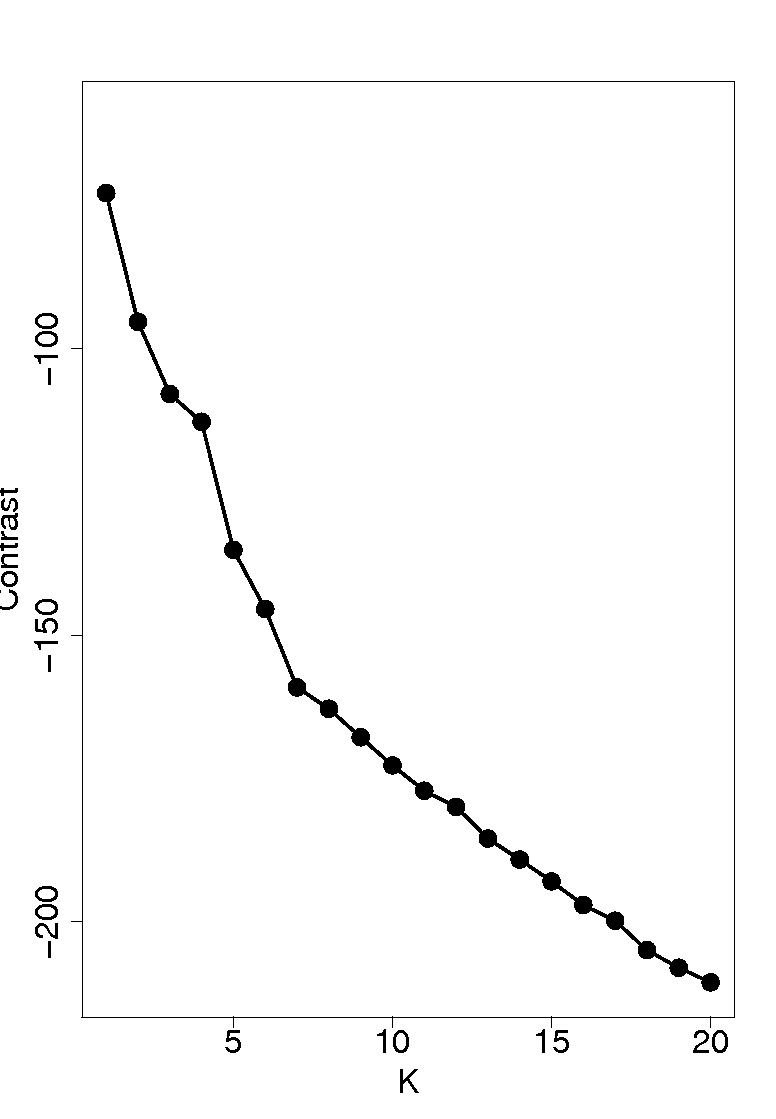
\epsfig{file = ../FIGURES/Bt474-J.ps, clip=, width=.5\textwidth,
	       height=.7\textheight} 
    	\onslide<3>
	      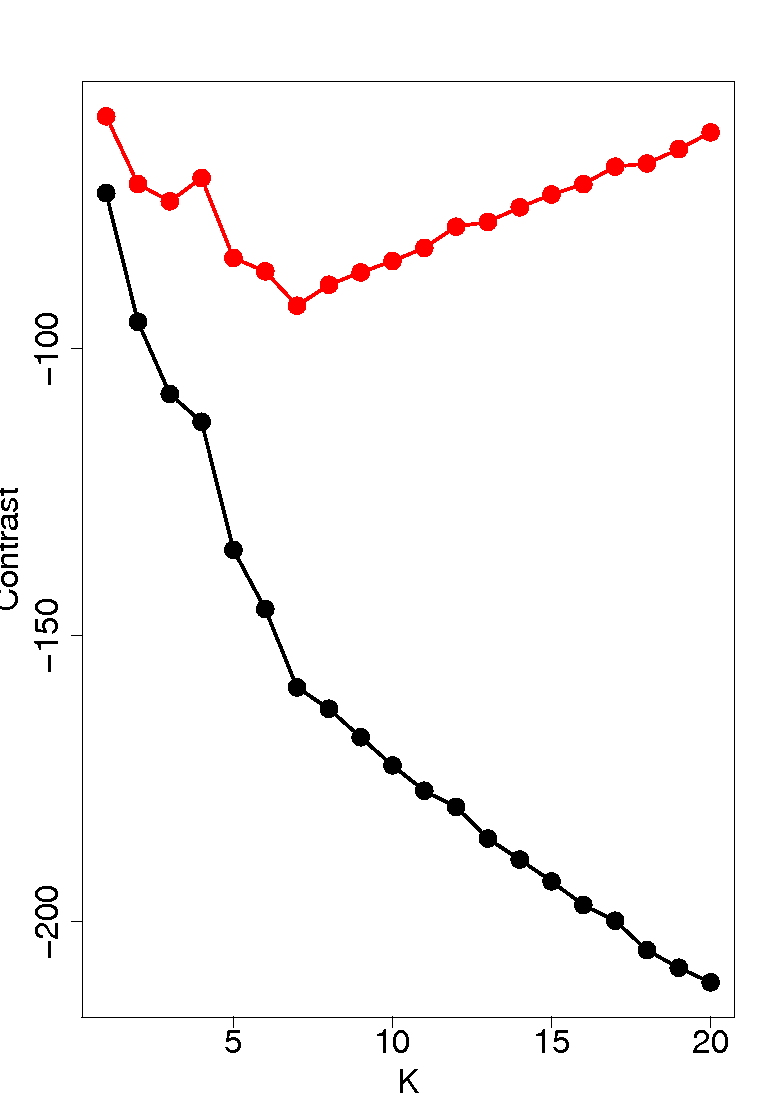
\epsfig{file = ../FIGURES/Bt474-JP.ps, clip=, width=.5\textwidth,
	       height=.7\textheight} 
    	\onslide<4->
	      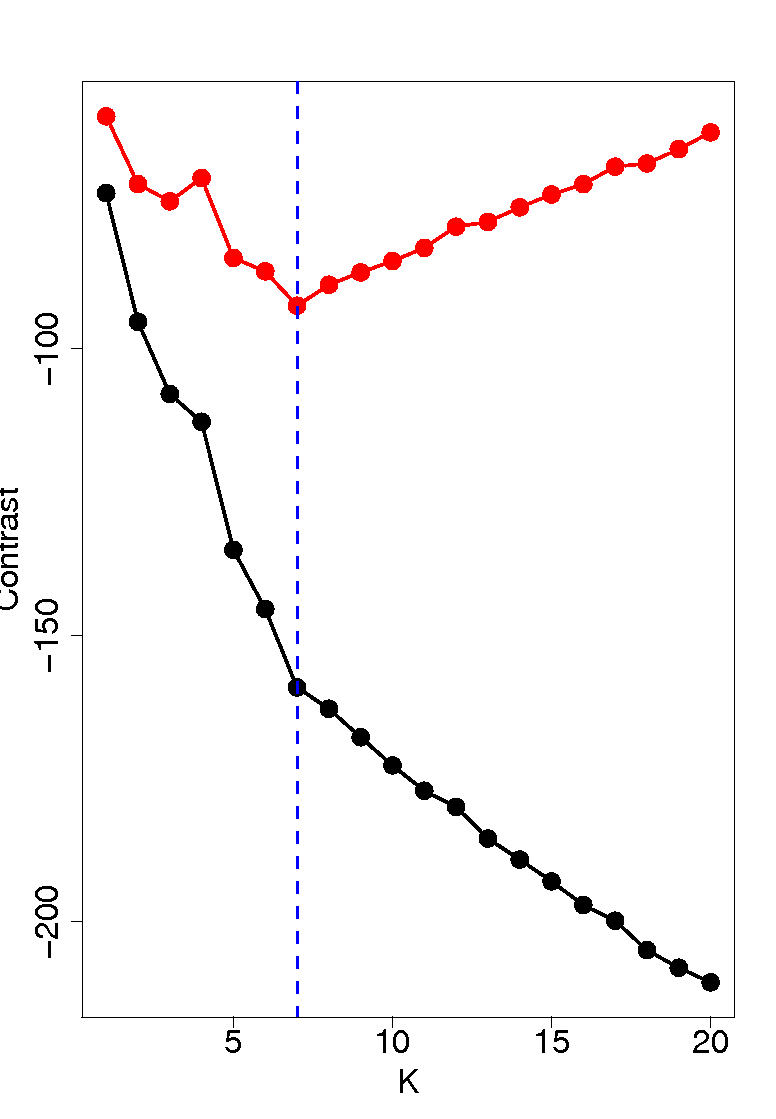
\epsfig{file = ../FIGURES/Bt474-JPM.ps, clip=, width=.5\textwidth,
	       height=.7\textheight} 
	    \end{overprint}
    \end{tabular} 
  \end{tabular} 

  \onslide+<5>{ 
    \vspace{-.5cm} An abundant literature has been developed
    (\refer{Leb05}, \refer{Lav05}, \refer{ZhS07}, ...) to insure that
    $\Pr\{\widehat{K} = K\} \rightarrow 1$ when $n \rightarrow \infty$
    or to approximate $p(K | \Ybf)$.  }
  
}

%====================================================================
\frame{\frametitle{Comparative study (for CGH)}

  Based on \emphase{manually annotated CGH profiles}, ROC curves can be drawn to compare the performances of a series methods, in terms of change-point detection (\refer{Hoc12}). \\
  \pause
  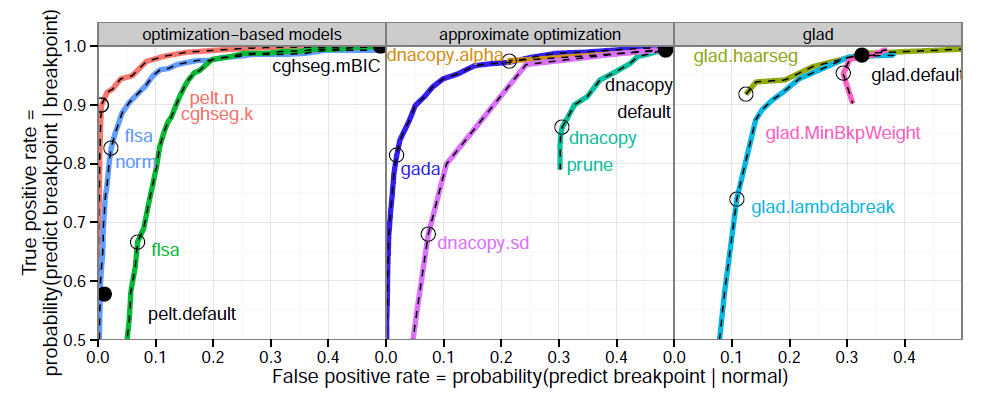
\epsfig{file = ../FIGURES/Hoc12-Fig3-3.eps, width=.95\textwidth}     \\
  \pause 
%   \vspace{-.5cm}
  \begin{itemize}
   \item DP and PELT clearly achieve the best performances.
   \item These two methods exactly the (penalized) likelihood maximization.
   \item But the choice of the number of segments remains an issue.
  \end{itemize}

 }
 
%====================================================================
\frame{\frametitle{Example: Breast cancer CGHarray}

  \vspace{-.5cm}
  \[
  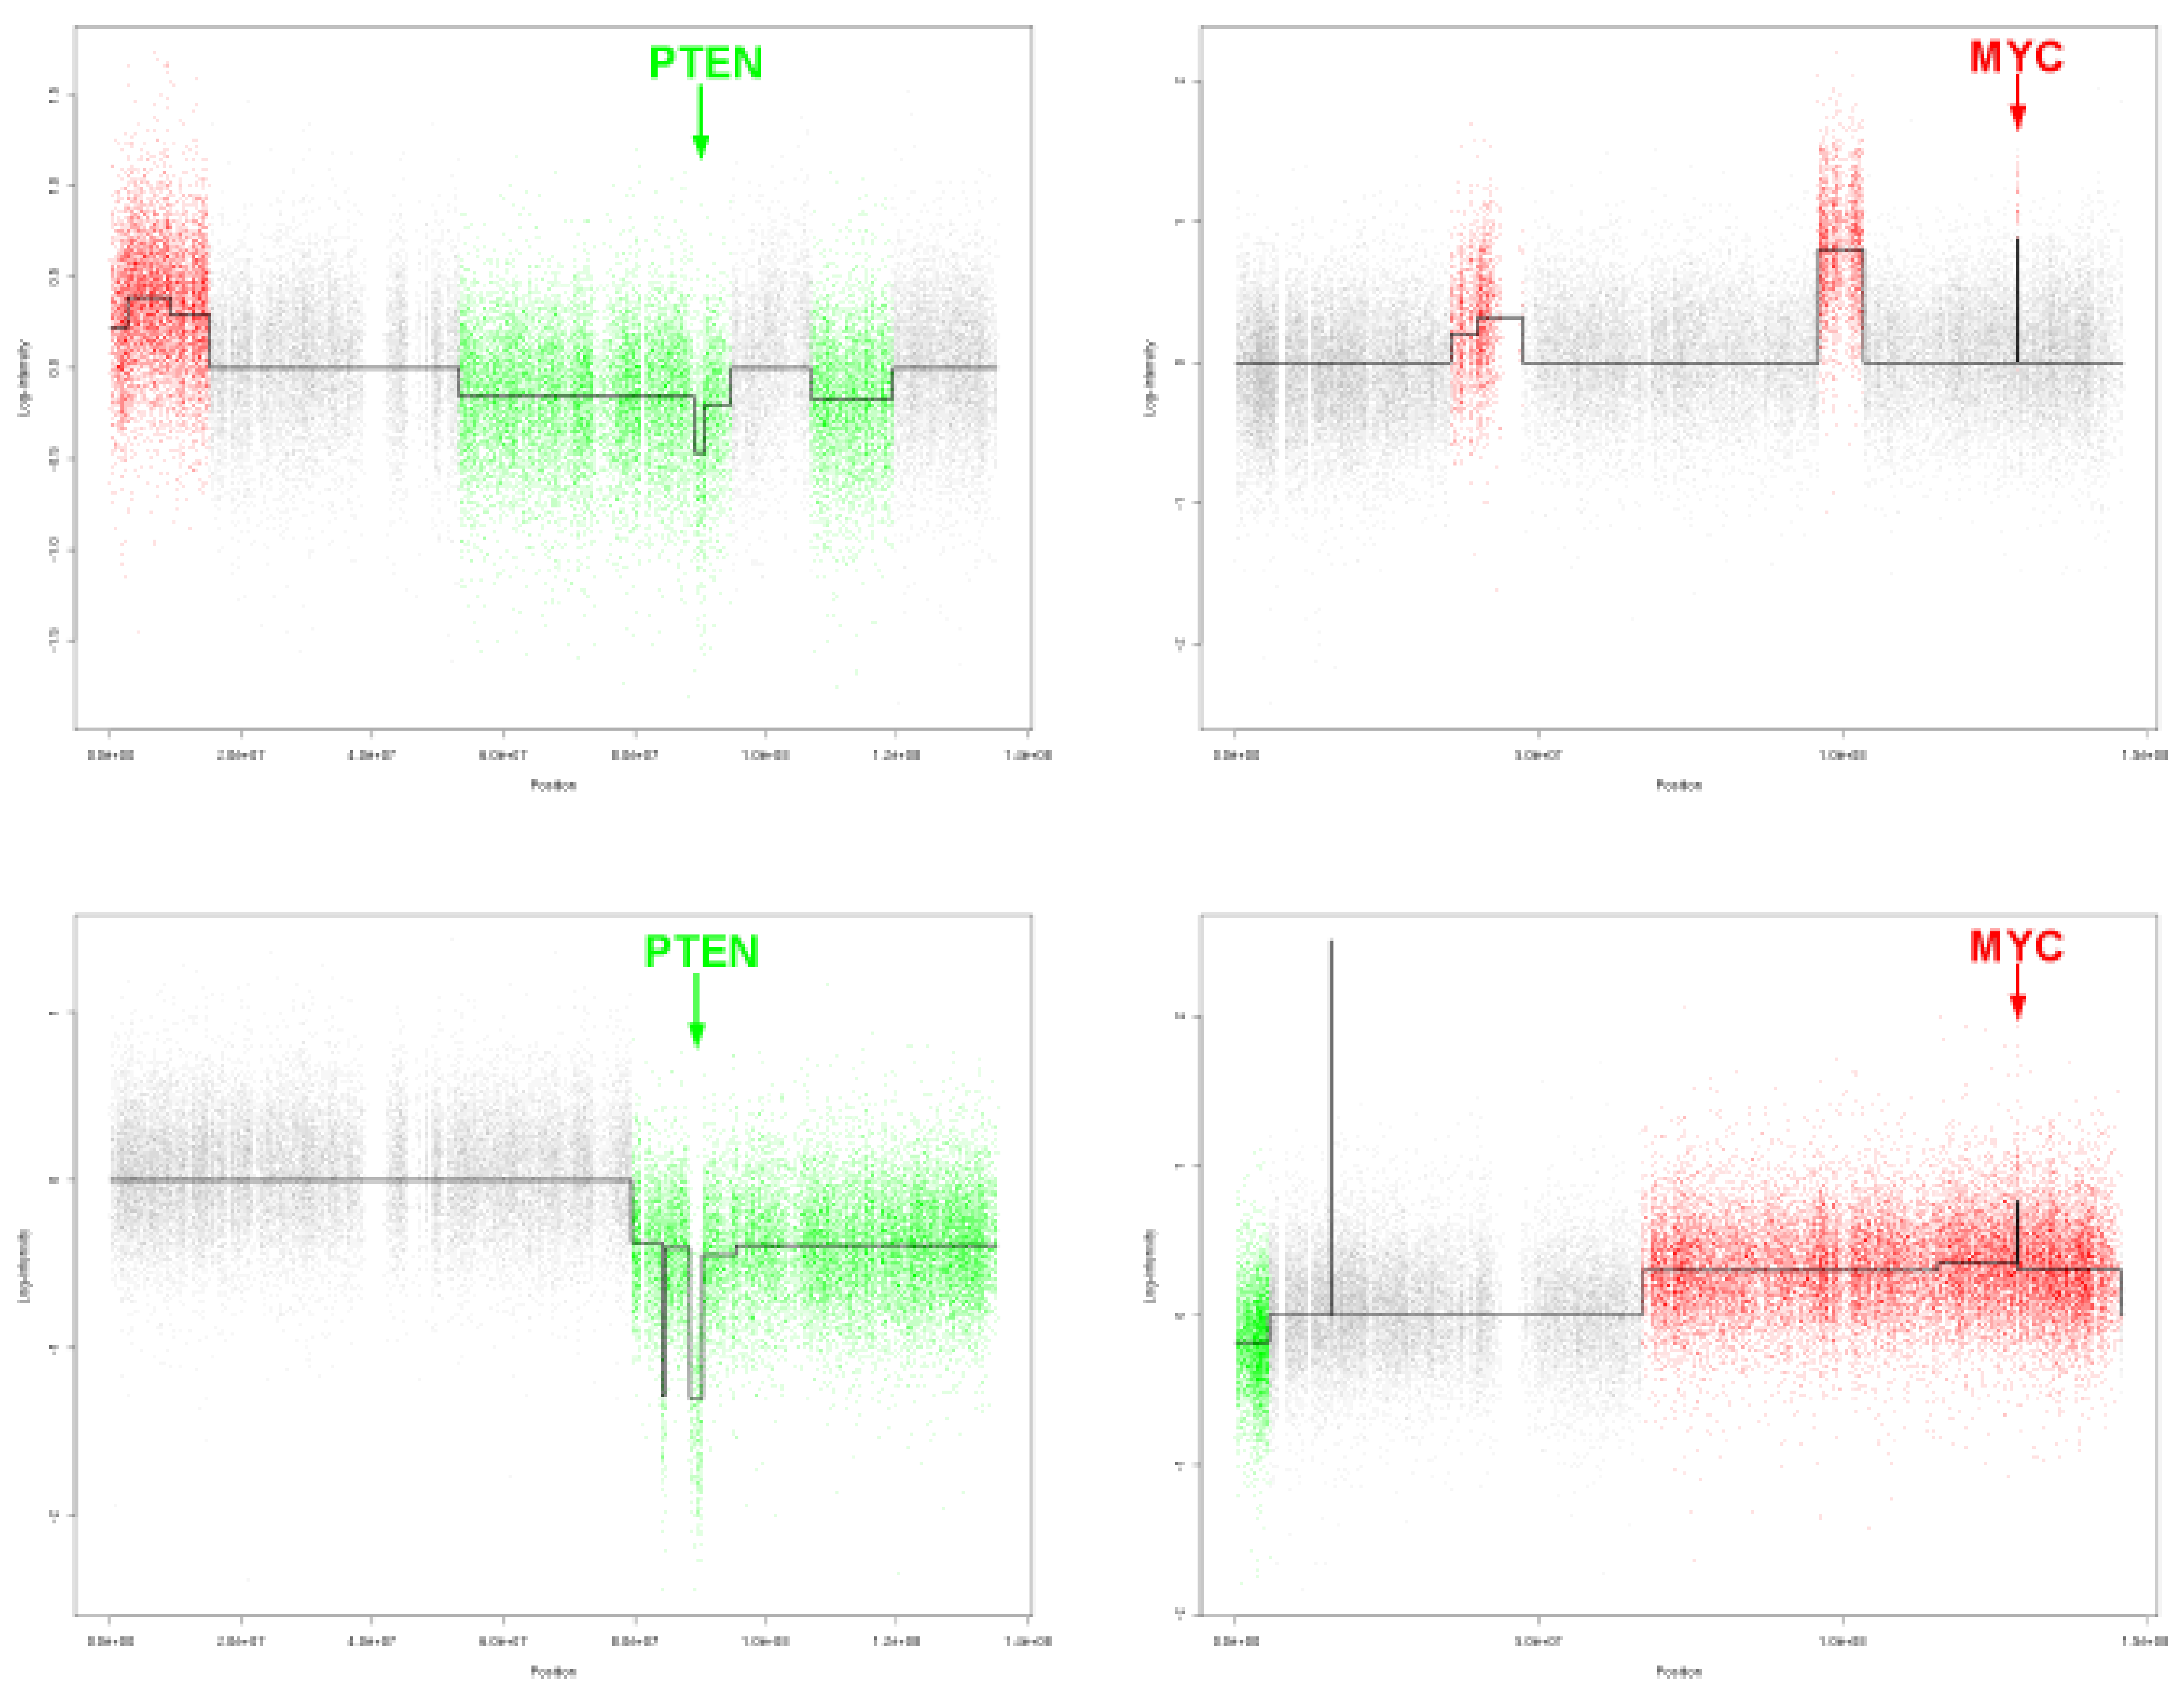
\epsfig{file = ../FIGURES/Rig10-Fig6-5.ps, height=.8\textheight,
    width=.8\textwidth} 
  \] 
  Chrom. 10 and 8 of two breast carcinomas (TNBC). \refer{Rig11} 
}\label{Page:BreastCancer}

%====================================================================
\subsection*{Comparing change-points}
%====================================================================
\frame{\frametitle{A bit further: comparing change-points}

  \paragraph{Change-point location.} No method described until now gives information about the \emphase{precision of the change point location $\tau_k$} (confidence or credibility interval).

  \pause\bigskip\bigskip
  \paragraph{Credibility interval.} A quadratic ($O(Kn^2)$) algorithm can be designed to compute the (exact) posterior distribution of the change points.	
  $$
  \epsfig{file=../FIGURES/Bayes-data.ps, clip=, width=1\textwidth, bburx=515, bbury=315, bbllx=0, bblly=210}
  $$

  }

%====================================================================
\frame{\frametitle{Change-point comparison}

  \begin{tabular}{cc}
    \hspace{-.5cm}
    \begin{tabular}{p{.5\textwidth}}
      \onslide+<1->{
        \paragraph{Change-point location}
        \begin{itemize}
        \item Comparison \textcolor{red}{posterior} vs \\
          \textcolor{blue}{'official' annotation}
        \end{itemize} 
	~\\
        }
      \onslide+<2->{
        \paragraph{Comparison}
        \begin{itemize}
        \item Posterior distribution under different conditions can be compared.
        \item Providing a statistical assessment of transcription starting sites variations.
        \end{itemize}
        ~\\ ~\\ ~\\ ~\\ ~\\
        }
    \end{tabular}
    & 
    \hspace{-1.3cm} 
    \begin{tabular}{p{.5\textwidth}}
      %\vspace{-.5cm}
      \begin{overprint}
        \onslide<1>
	\epsfig{file=../FIGURES/Bayes-data.ps, clip=, width=.5\textwidth, height=.9\textheight}
%         \includegraphics[width=.5\textwidth, height=.9\textheight]{../FIGURES/Bayes-data} 
        \onslide<2->
	\epsfig{file=../FIGURES/compa-end.ps, clip=, width=.5\textwidth, height=.4\textheight, bbllx=40, bblly=50, bburx=500, bbury=210} 
	\\ ~\\ ~\\
	\ra EBS R package available on CRAN
%         \includegraphics[width=.5\textwidth, height=.9\textheight]{../FIGURES/compa-end}
      \end{overprint}
    \end{tabular}
  \end{tabular}
}

%====================================================================
\subsection*{Calling}
%====================================================================
\frame{\frametitle{What about calling?}

  \paragraph{Calling.} We'd like segments of same type ('normal',
  'loss', gain', {\sl etc.}) to be gathered into groups \ra
  classification problem.

  \bigskip
  \begin{tabular}{cc}
    \hspace{-0.5cm}
    \pause
    \begin{tabular}{p{.5\textwidth}}
      Pure segmentation \\
      \epsfig{file = ../FIGURES/FigSegClas-1.eps, clip=,
        width=0.45\textwidth, height=0.25\textwidth}
    \end{tabular} 
    &
    \hspace{-1cm}
    \pause
    \begin{tabular}{p{.5\textwidth}}
      Segmentation + classification \\
      \epsfig{file = ../FIGURES/FigSegClas-2.eps, clip=,
        width=0.45\textwidth, height=0.25\textwidth}
    \end{tabular}
  \end{tabular}

  \bigskip\pause
  \paragraph{How to do this.}
  \begin{itemize}
  \item Either combine the segmentation model with a mixture model 
    (\refer{PRL07}). 
  \item Or use HMM (see slide  \ref{Page:HMM}).
  \end{itemize}
  }

%====================================================================
%====================================================================
\section{Segmentation of multiple profiles}
\frame{\frametitle{Segmentation of multiple profiles}}
%====================================================================
\frame{\frametitle{Multiple profiles}
  
  \begin{tabular}{cc}
    \begin{tabular}{p{6cm}}
      Cancer studies often involve CGH profiles of numerous
      patients ($m \approx 100$). \\
      \bigskip
      Even when having the same disease, patients generally
      \emphase{do not have common breakpoints}.\\
      \bigskip
      Simultaneous analysis of all profiles $\{Y_{it}\}$ allows
      to \emphase{correct for artifacts} such as probe effect.\\
        \bigskip
      \refer{PLB11}
    \end{tabular}    
    &
    \begin{tabular}{p{6cm}}
      \hspace{-.75cm}
      \epsfig{file = ../FIGURES/nakao-mat.txt-MixSeg-V2.eps, bbllx=90,
      bblly=220, bburx=380, bbury=590, clip=, scale=.5}
    \end{tabular}
  \end{tabular}
  }

%====================================================================
\subsection*{Statistical model}
%====================================================================
\frame{\frametitle{Statistical model}

  \paragraph{Notation.}
  \begin{itemize}
  \item $Y_{it} = $ signal for patient $i$ ($i = 1..m$) at position
    $t$ ($t = 1..n$);
  \item $K_i = $ number of segments of patient $i$;
  \item $I_{ik} = k$-th segment of patient $i$ ($k = 1.. K_i$).
  \end{itemize}

  \bigskip\pause
  \paragraph{Model.} Data are independent, 
  $$
  \text{if }t \in I_{ik}, \qquad Y_{it} \sim \Ncal(\mu_{ik} + \beta_t,
  \sigma^2)
  $$
  where $\beta_t$ stands for the \emphase{probe effect} at position
  $t$.  

  \bigskip\pause
  \paragraph{Remark.} The model can be written as a \emphase{linear
    model}:
  $$
  \Ybf = \Tbf  \mubf + \Xbf \betabf + \Ebf
  $$
  ... where the segmentation matrix $\Tbf$ is unknown.
}\label{Page:MultiModel}

%====================================================================
\subsection*{Inference}
%================================================\pause====================
\frame{\frametitle{Statistical inference}

  \paragraph{Segmentation.} DP can be generalized (2-stage DP
  algorithm) to perform the segmentation of multiple profiles with a
  fixed total number of segments $K_+ = \sum_i K_i$.

  \bigskip\bigskip\pause
  \paragraph{Model selection.} Criteria used for one single profile
  can be generalized as well.

  \bigskip\bigskip\pause
  \paragraph{Parameter estimation.} The mean of each segments
  ($\mu_{ik}$) and the probe effect ($\beta_t$) must can be estimated
  in an iterative way:
  \begin{eqnarray*}
    \emphase{\mu^{h+1}_{ik}}  & = & \arg\min_{\mu_{ik}} \sum_i \sum_k \sum_{t \in
      I_{ik}} (Y_{it} - \mu_{ik} - \emphase{\beta^h_t})^2, \\
    \emphase{\beta_t^{h+1}} & = & \arg\min_{\beta_t} \sum_i \sum_k \sum_{t \in
      I_{ik}} (Y_{it} - \emphase{\mu^{h+1}_{ik}} - \beta_t)^2. \\
  \end{eqnarray*}

}

%====================================================================
\subsection*{CGHseg R-package}
%====================================================================
\frame{\frametitle{CGHseg R-Package} 

  \paragraph{CGHseg} is an R package dedicated to the analysis of
  Comparative Genomic Hybridization (\refer{PLH11}). 
  
  \bigskip\pause
  \paragraph{Linear model framework:} 
 
  \medskip
  \begin{tabular}{p{.2\textwidth}p{.35\textwidth}p{.35\textwidth}}
%     \emphase{Task} & \emphase{Representation} & \emphase{Model} \\   
%     \hline
%     \\
    \emphase{Segmentation} & regression on unknown $\Tbf$: &
    $\displaystyle{\Ybf = \Tbf \mubf + \Ebf}$ \pause \\ 
    \\
    \emphase{Correction} & fixed covariates effect: $\betabf$ &
    $\displaystyle{\Ybf = \Tbf \mubf + \Xbf \betabf + \Ebf}$ \pause \\  
    \\
    \emphase{\sl Correlation}\footnote{\refer{PLB11}} & {\sl random
      probe effect: $\Ubf$}  & 
    $\displaystyle{\sl \Ybf = \Tbf \mubf + \Zbf \Ubf + \Ebf}$  \pause \\ 
    \\
    \emphase{Calling} & cross-tabulation table $\Cbf$: &
    $\displaystyle{\Ybf = \Tbf \Cbf \mbf + \Ebf}$ \pause \\
    \\
    \emphase{Combinations} 
    & fixed + random effects: &
    $\displaystyle{\Ybf = \Tbf \mubf + \Xbf \betabf + \Zbf \Ubf + \Ebf}$ \\
    & fixed effects + calling: &
    $\displaystyle{\Ybf = \Tbf \Cbf \mbf + \Xbf \betabf + \Ebf}$  \\
  \end{tabular}
}


%====================================================================
\frame{\frametitle{An example of combination}

  \begin{tabular}{ccc}
    \onslide+<1->{\textcolor{red}{Segmentation}
      % +\textcolor{green}{calling}
    }
    & 
    \onslide+<2->{+ \textcolor{blue}{fixed effects} }
    & 
    \onslide+<3->{$\Ybf = \textcolor{red}{\Tbf} 
      %\textcolor{green}{\Cbf} 
      \mbf + \textcolor{blue}{\Xbf} \betabf + \Ebf$  }
    \\
    % \epsfig{file = ../FIGURES/PLH11-V1-Fig1.eps, clip=, angle=270,
    %   bbllx=10, bblly=0, bburx=300, bbury=840, scale=0.4}        
    \onslide+<1->{\epsfig{file = ../FIGURES/PLH11-V1-Fig1.eps, clip=,
        angle=270, bbllx=33, bblly=34, bburx=282, bbury=272,
        scale=0.4}}   
    & 
    \onslide+<2->{\epsfig{file = ../FIGURES/PLH11-V1-Fig1.eps,
        clip=, angle=270, bbllx=33, bblly=302, bburx=282, bbury=540,
        scale=0.4}} 
    & 
    \onslide+<3->{\epsfig{file = ../FIGURES/PLH11-V1-Fig1.eps, clip=,
        angle=270, bbllx=33, bblly=571, bburx=282, bbury=810,
        scale=0.4}}         
  \end{tabular}

  \bigskip
  \onslide+<4->{
    \begin{itemize}
    \item \emphase{Correction:} functional versions (spline, wavelets)
      for the probe effect.
    \item Several model selection criteria; Default = modified BIC.
%    \item \emphase{Presentation} at
%      \url{www.agrocampus-ouest.fr/math/useR-2009/}
    \item \emphase{\tt cran.r-project.org/web/packages/cghseg/index.html}
    \end{itemize}
  }
  
}

%====================================================================
\frame{\frametitle{Some simulations}

  \vspace{-0.5cm}
  \begin{tabular}{cc}
    \hspace{-0.5cm}
    \begin{tabular}{p{.5\textwidth}}
      Correction and calling improve
      \begin{itemize}
      \item the estimation of $K$, 
      \item the breakpoint detection (FDR / FNR), 
      \item the  recovery of the true signal.
      \end{itemize}
      
      \bigskip
      \paragraph{Calling:} yes = --, no = - -

      \bigskip
      \paragraph{Correction:} \\
      $\blacksquare =$ no correction, \\
      \textcolor{red}{$\bullet = $ position  specific}, \\
      \textcolor{blue}{$\triangle =$ spline}, \\
      \textcolor{green}{$\diamond =$ wavelet}, \\
      \textcolor{orange}{$\circ =$ CBS} 
    \end{tabular}
    &
    \hspace{-1cm}
    \begin{tabular}{p{.5\textwidth}}
      \epsfig{file = ../FIGURES/PLH11-V1-Fig2.eps, clip=,
        width=.5\textwidth, height=0.85\textheight}        
    \end{tabular}
  \end{tabular}

  }

%====================================================================
\section{Hidden Markov models}
\frame{\frametitle{Hidden Markov models} \pause

  \vspace{-0.5cm}
  \begin{tabular}{cc}
    \hspace{-.5cm}
    \begin{tabular}{p{.5\textwidth}}
    {\paragraph{Statistical model.} }
      \begin{itemize}
      \item {$t = 1..n$ probes (positions) are observed. \\~}
      \item {A (Markov) succession of \emphase{labels $Z_t$}
          ('loss', '\textcolor{red}{normal}',
          '\textcolor{darkgreen}{gain}') is associated with each probe. \\~}
      \item {The distribution of the \emphase{observed signal
          $Y_t$} depends on the label. \\~}
      \item {The labels are \emphase{hidden}.}
      \end{itemize}
    \end{tabular}
    &    \hspace{-1cm}
    \begin{tabular}{p{.5\textwidth}}
        $\qquad \qquad (Z_t)\sim MC(\pi)$ \\
        $\text{~~~~~if } Z_t=\textcolor{red}{k}, \quad Y_t = \textcolor{red}{\mu_k} + E_t$ \\
        \epsfig{file=\figSimHMM/SimHMM_n100_Q3_ZX.eps,
          width=0.4\textwidth, height=0.7\textheight, angle=270, clip=}
    \end{tabular}
  \end{tabular} 
}

\label{Page:HMM}
%====================================================================

%====================================================================
\frame{\frametitle{Statistical model}

  \onslide+<1->{
    \paragraph{Hidden labels.} $(Z_t)$ is a Markov chain:
    \begin{itemize}
    \item $Z_t \in \emphase{\{1..Q\}}$, e.g. $Q = 3$ for
      $\{$'loss', 'normal', 'gain'$\}$;
    \item The label of a probe \emphase{depends on the label of the
        preceding} probe:
      $$
      \text{transition probability} \quad \pi_{q\ell} = 
      \Pr\{Z_t = \ell | Z_{t-1} = q\}
      $$
    \end{itemize}
    }
    
    \onslide+<2->{
      \bigskip
      \paragraph{Observed signal.} $(Y_t)$ are independent, given the
      labels $(Z_t)$:
      $$
      \text{if } Z_t = q: \qquad
      Y_t \sim \Ncal(\mu_q, \sigma^2_{(q)})
      \qquad \text{or} \qquad
      Y_t \sim \Pcal(\mu_q).
      $$
    }
    
    \paragraph{Graphical model representation.}
    \begin{overprint}
      \onslide<1>
      $$
      \epsfig{file=../FIGURES/GM-HMM-ZY.eps,
        bbllx=0, bblly=464, bburx=660, bbury=540,
        width=0.7\textwidth, clip=}
      $$
      \onslide<2>
      $$
      \epsfig{file=../FIGURES/GM-HMM-ZY.eps,
        bbllx=0, bblly=335, bburx=660, bbury=540,
        width=0.7\textwidth, clip=}
      $$
    \end{overprint}
  }

%====================================================================
\frame{\frametitle{Parameter inference}

  \paragraph{Incomplete data model.} The likelihood of the observed data is not managable:
  $$
  P(\Ybf) = \sum_{\Zbf} P(\Ybf | \Zbf) P(\Zbf) 
  $$
  Parameter inference would be easy if the labels $Z_t)$ where known, that is to deal with the 'complete' data likelihood
  $$
  P(\Ybf, \Zbf) = P(\Ybf | \Zbf) P(\Zbf). 
  $$
  
  \bigskip\pause
  \paragraph{E-M algorithm.} The most common strategy consist in, iteratively,
  \begin{itemize}
  \item \emphase{E-step:} retrieve the missing labels $\Zbf$ based on the observed data $\Ybf$ and a current value of the parameter estimates;
  \item \emphase{M-step:} update the parameter estimates using the data and the pseudo-labels
  \end{itemize}
  }
  
%====================================================================
\frame{\frametitle{Parameter inference (cont'd)}
  
  \paragraph{More precisely.}
  \begin{itemize}
  \item \emphase{E-step:} Compute the conditional distribution of the labels $\Zbf$ given the observed data $\Ybf$ to get (among other things)
    $$
    \tau_{tq} = \Pr\{Z_t = q \;|\; \Ybf\}.
    $$
    \ra famous 'forward-backward' algorithm with complexity $O(nK�)$.
  \item \pause \emphase{M-step:} Estimate the parameters based the
    infered labels, e.g.
    \begin{eqnarray*}
    \widehat{\mu}_q & = & \sum_t \tau_{tq} Y_t \left/ \sum_t \tau_{tq} \right. \\
    \widehat{\pi}(q, \ell) & \propto & \sum_t \Pr\{Z_{t-1}=k, Z_t = \ell | \Ybf\}.
    \end{eqnarray*}
  \end{itemize}
  \refer{DLR77}, \refer{CMR05}, \refer{DEK99}
  }

%====================================================================
\frame{\frametitle{Calling vs segmentation}

  \onslide+<1->{
    Calling = local inference / segmentation = global inference.
  }
  
  \bigskip
  \begin{tabular}{cc}
    \hspace{-0.5cm}
    \begin{tabular}{p{.5\textwidth}}
      \onslide+<2->{
        \paragraph{Probe classification: MAP rule.} 
        The $\tau_{tq}$ can provide \emphase{maximum a posteriori}
        classification:
        $$
        \widehat{Z}_t = \arg\max_q \tau_{tq}.
        $$ \\
      }
      \onslide+<3->{
        \paragraph{Segmentation: Most probable hidden path.} The succession of the
        MAP $(\widehat{Z}_t)$ is \emphase{not} the most probable
        hidden path:
        $$
        \widehat{\Zbf} = \arg\max_{\Zbf} P(\Zbf|\Ybf) \neq
        (\widehat{Z}_t) 
        $$
        % \begin{eqnarray*}
        %   \widehat{\Zbf} & = & \arg\max_{\Zbf} P(\Zbf|\Ybf) \\
        %   & \neq & (\widehat{Z}_t) 
        % \end{eqnarray*}
      }
    \end{tabular}
    &
    \hspace{-1cm}
    \begin{tabular}{p{.5\textwidth}}
      \begin{overprint}
        \onslide<1> 
        \epsfig{file=\figSimHMM/SimHMM_n100_Q3_X.eps,
          width=0.4\textwidth, height=0.7\textheight, angle=270, clip=}
        \onslide<2> 
        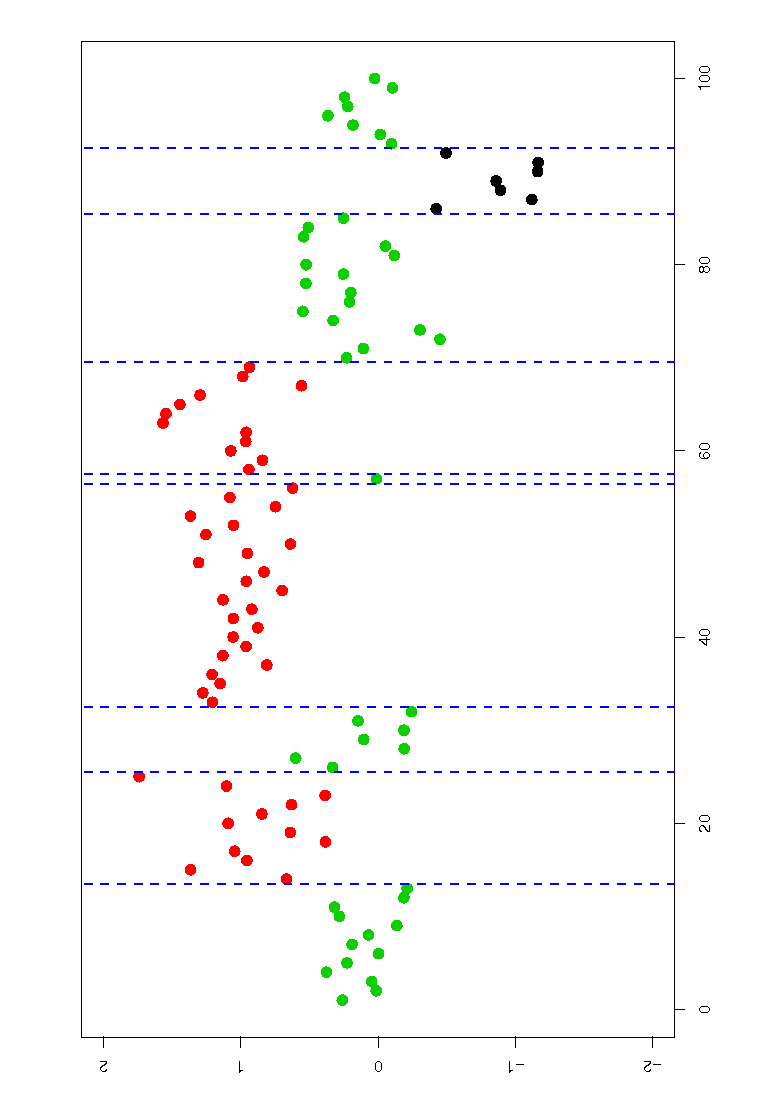
\epsfig{file=\figSimHMM/SimHMM_n100_Q3_ZmapXT.eps,
          width=0.4\textwidth, height=0.7\textheight, angle=270, clip=}
        \onslide<3> 
        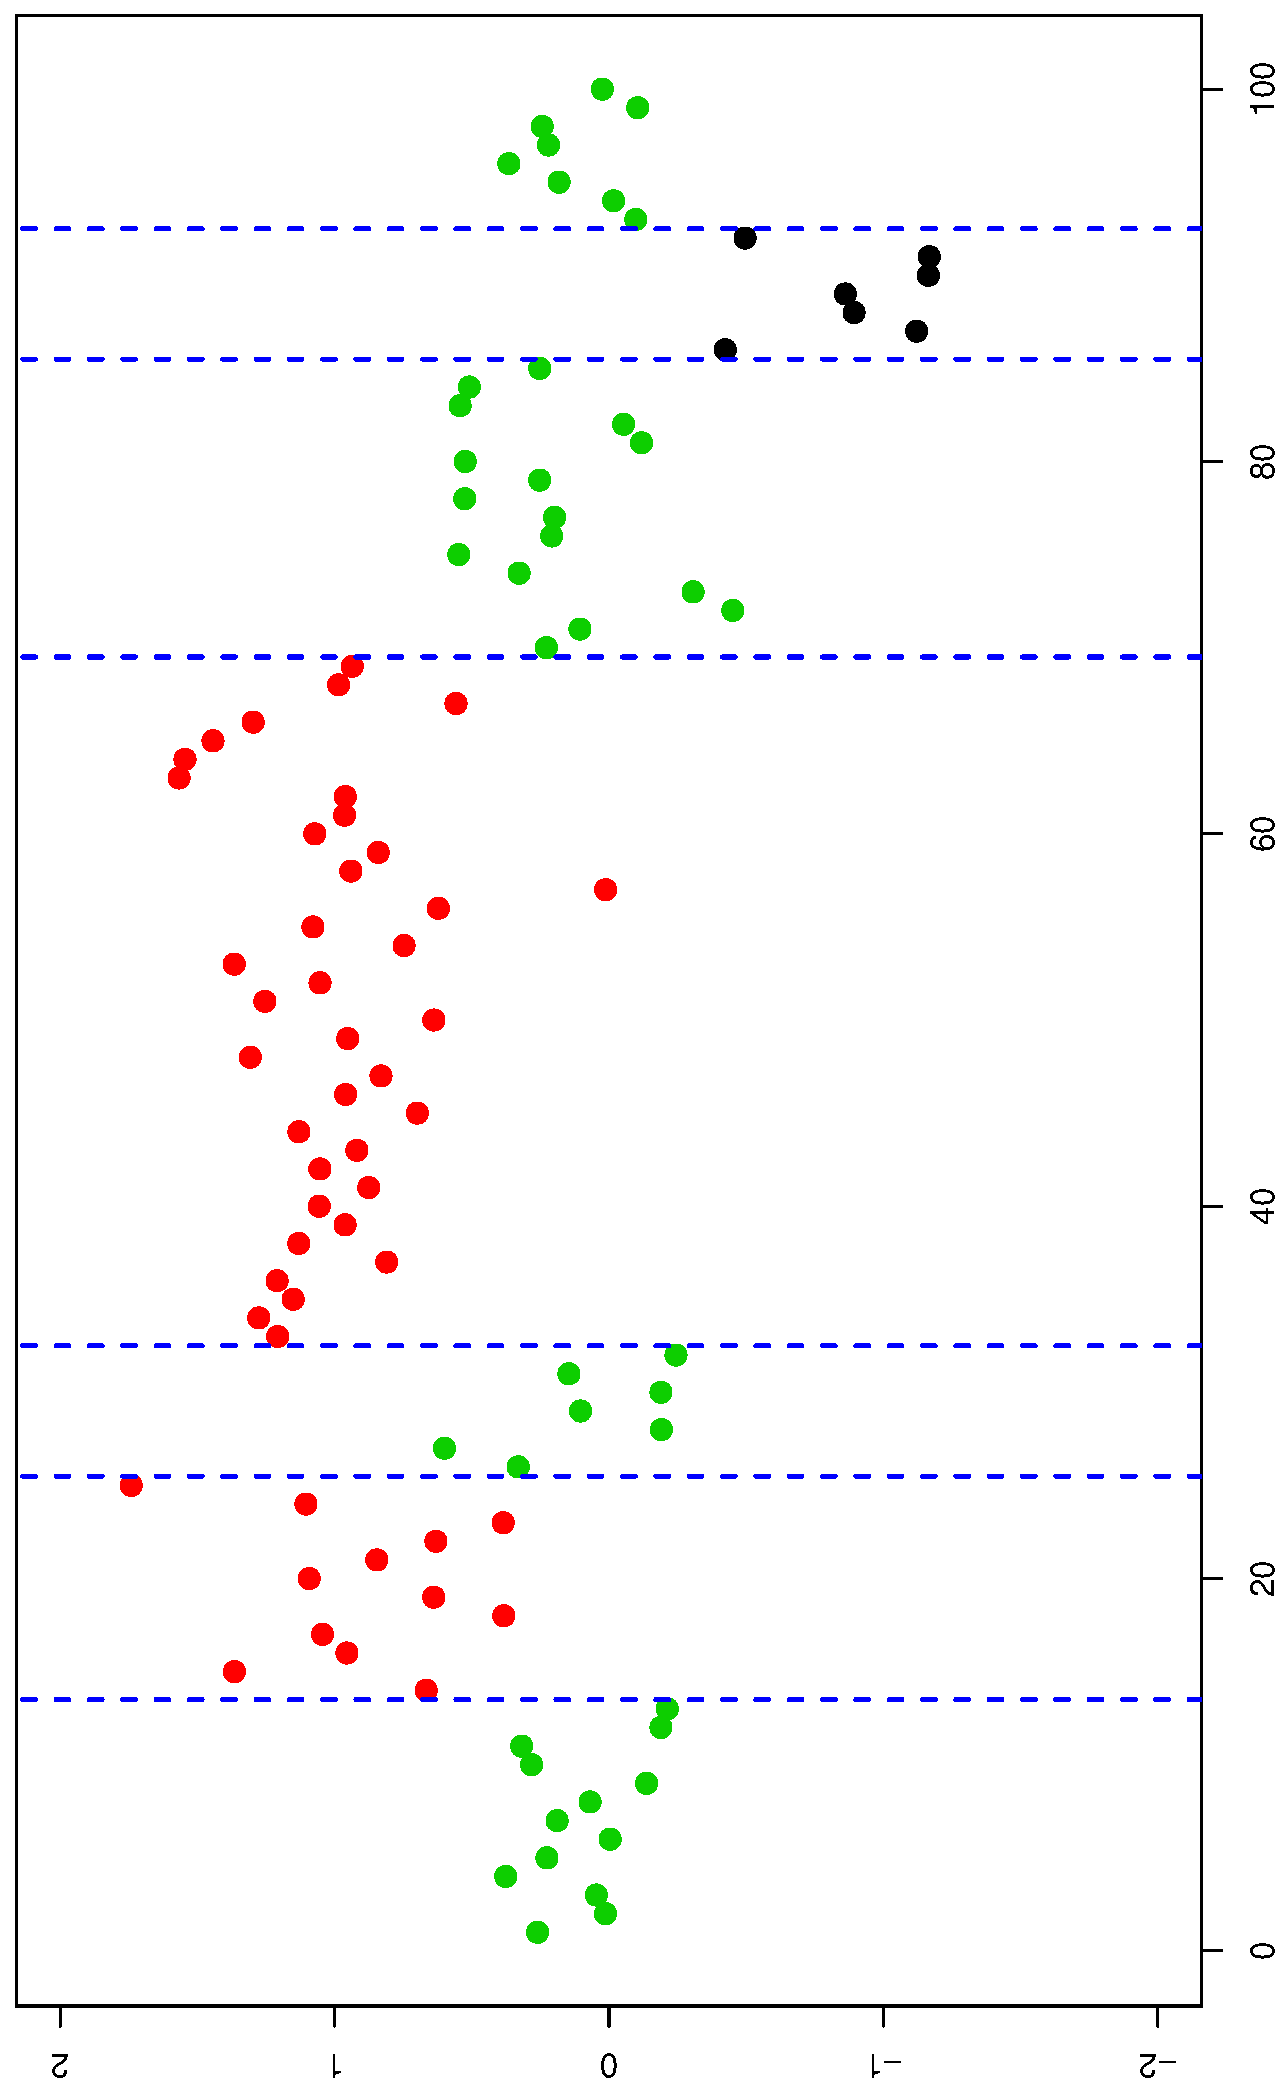
\epsfig{file=\figSimHMM/SimHMM_n100_Q3_ZvitXT.eps,
          width=0.4\textwidth, height=0.7\textheight, angle=270, clip=}
      \end{overprint}
    \end{tabular}
  \end{tabular}
  
  }

%====================================================================
\frame{\frametitle{Issues}

  \paragraph{Algorithmics.} 
  \begin{itemize}
  \item The conditional distribution of the labels given the
    observation $\emphase{P(\Zbf | \Ybf)}$ is not explicit;
  \item But it can be computed \emphase{in a linear time $O(nK^2)$}
    with the forward-backward algorithm.
  % \item The most probable hidden path $\widehat{\Zbf} = \arg\max
  %   P(\Zbf | \Ybf)$ can be computed with the same complexity with
  %   the Viterbi algorithm.
  \end{itemize}
  
  \bigskip\pause
  \paragraph{Statistics.}
  \begin{itemize}
  \item The E-M algorithm aims at computing the maximum-likelihood
    estimates;
  \item But its behavior strongly depends on the starting point...
  \item The Markov assumption has some consequences on the
    distribution of the length of the segments.
  \end{itemize}
  
  \bigskip\pause
  \paragraph{Model selection.}
  \begin{itemize}
  \item The number of hidden classes $Q$ is unknown;
  \item But is often chosen with standard criteria, such as BIC.
  \end{itemize}
}


%====================================================================
\subsection*{Applications}
%====================================================================
\frame{\frametitle{Application to CGH}
  
  HMM have been used early for aCGH analysis (\refer{FSP04})
  
  \bigskip
  \begin{tabular}{cc}
    \hspace{-0.5cm}
    \begin{tabular}{p{.5\textwidth}}
      \onslide+<2->{
        \paragraph{BT474 cell lines.}  \\
        Data from chromosome 9: \\
      }
      \onslide+<3->{
        $\begin{array}{rrrr}
          & \text{\textcolor{red}{gain}} & \text{\textcolor{black}{normal}} &
          \text{\textcolor{darkgreen}{loss}} \\
          \hline
          \widehat{\mu}_q & 1.18 & 0.19 & -0.92 \\
          \hline
          & 87.6 & 12.4 & 0.0 \\
          \widehat{\pi}_{q\ell} & 2.0 & 98.0 & 0.0 \\
          & 4.0 & 0.0 & 96.0 \\
          \hline
          \widehat{\sigma}^2 & & 0.12 & \\
        \end{array}$ \\
      }
    \end{tabular}
    &
    \hspace{-1.5cm}
    \begin{tabular}{p{.5\textwidth}}
      \begin{overprint}
        \onslide<2> 
        \epsfig{file = ../FIGURES/Bt474_c9.eps, clip=,
          width=.35\textwidth, angle=270} 
        \onslide<3> 
        \epsfig{file = ../FIGURES/Bt474_c9_hmm_homo_Q3_vit.eps, clip=,
          width=.35\textwidth, angle=270} 
      \end{overprint}
    \end{tabular}
  \end{tabular}

  \pause
  \paragraph{Remark.} Because of the sensitivity of E-M to the
  starting point, several trials have been needed to get meaningful
  results. \\
  \ra A clever initialization procedure is needed.
%   
}

%====================================================================
\frame{\frametitle{Other arrays}

  HMM can be used for various tiling arrays: transcriptome, ChIP. \\
  ~\\
  \paragraph{Example.} Tiling array comparing transcript abundance between 2 conditions. \\

  %\vspace{-0.5cm}
  \begin{tabular}{cc}
    \hspace{-0.5cm}
    \begin{tabular}{p{.4\textwidth}}
	~\\
	Emission distribution = (mixture of) bivariate Gaussian (\refer{BMB11}). \\
	~\\
	\onslide+<2->{HMM can account for the available annotation ... or be used to question it. \\ ~\\ ~\\ ~\\ ~\\}
    \end{tabular}
    &
    \hspace{-.5cm}
    \begin{tabular}{p{.5\textwidth}}
      \begin{overprint}
       \onslide<1>
       \epsfig{file=../FIGURES/Ber12-Fig510.eps, clip=, width=.5\textwidth}
       \onslide<2>
       \epsfig{file=../FIGURES/Ber12-Fig523.eps, clip=, width=.5\textwidth} \\
	~\\
       HMMannot R package on CRAN
      \end{overprint}
    \end{tabular}
  \end{tabular} \\

}


%====================================================================
%====================================================================
\section{Segmentation of multiple profiles}
\frame{\frametitle{Segmentation of multiple profiles}}
%====================================================================

%====================================================================
\subsection*{Modeling Dependency}
%====================================================================
\frame{\frametitle{Multiple profiles}

  \paragraph{General model several profiles.} 
  \begin{itemize}
  \item Consider $m$ individuals $(i = 1..m$) with hidden labels $\Zbf_i = (Z_{it})$.
%   \item Observe a profile $\Ybf_i$ for each of them or for a series of couples $\Ybf_{ij}$.
  \end{itemize}
  
   \bigskip \bigskip \pause
  \paragraph{Dependency between the hidden labels.} 
  The hidden labels underlying each observed profile can not be considered as independent
  \begin{itemize}
   \item either because of the experimental design
   \item or because of the genetic proximity between the individuals.
  \end{itemize}

}

%====================================================================
\frame{\frametitle{Comparative experiments}
  
   \paragraph{Comparing 3 individuals via 3 arrays.} CGH is a comparative technology.
   
   %\vspace{-0.5cm}
   \begin{tabular}{ccc}
    \hspace{-0.5cm}
    \begin{tabular}{p{.3\textwidth}}
       \epsfig{file=../FIGURES/CGHcomp-Ydiff.eps, clip=, width=.3\textwidth, height=.7\textheight}
    \end{tabular} \pause
    &
    \hspace{-0.5cm}
    \begin{tabular}{p{.3\textwidth}}
       \epsfig{file=../FIGURES/CGHcomp-Zdiff.eps, clip=, width=.3\textwidth, height=.7\textheight}
    \end{tabular} \pause
    &
    \hspace{-0.5cm}
    \begin{tabular}{p{.3\textwidth}}
       \epsfig{file=../FIGURES/CGHcomp-Z.eps, clip=, width=.3\textwidth, height=.7\textheight}
    \end{tabular}
  \end{tabular}

}

%====================================================================
\frame{\frametitle{Comparative experiments (cont'd)}
  
   \paragraph{Consistency.} HMM inference can not be performed independently because hidden labels of each individuals have to be consistent across the profiles.
   
   \bigskip \pause
   \paragraph{Graphical model.}
   $$
   \epsfig{file=../FIGURES/Wan13-GMcomp.eps, width=.7\textwidth} \pause
   $$
   Although hidden labels are independent a priori, they are dependent conditional on the observed profiles. \Refer{Wang, 2013}

}

%====================================================================
\frame{\frametitle{Accounting for genetic similarity}

   \paragraph{Accounting for genetic similarity.} Individuals may share common ancestors. Denote $d(i, j)$ the genetic distance between individual $i$ and $j$.

   \pause  \bigskip
   \paragraph{Graphical model.} Hidden labels are dependent a priori (even for non-comparative design).
   $$
   \epsfig{file=../FIGURES/Wan13-GMdist.eps, width=.7\textwidth}
   $$
   e.g.
   $
   \Pr\{Z_{i, t+1} = \ell, Z_{j, t+1} = \ell' | Z_{i, t} = k, Z_{j, t} = k'\} \propto \pi(k, \ell) \pi(k', \ell') \rho^{-\delta_{\ell \ell'}d(i, j)}.
   $
}

%====================================================================
\subsection*{Inference}
%====================================================================
\frame{\frametitle{Inference}

  \paragraph{Problem.} We now have to deal with a series of hidden labels $\Zbf_i$ ($i = 1, \dots m)$ with corresponding individuals profiles $\Ybf_i$ or comparisons $\Ybf_{ij}$
  
  \bigskip \bigskip \pause
  \paragraph{Direct strategy.} The set of all hidden labels $Z^t = (Z_{1t}, \dots Z_{mt})$ is still a Markov chain so the regular EM algorithm applies. \\
  ... but the state-space of $Z^t$ as dimension $Q^m$ \ra intractable even for intermediate population size $m$.
     
   \pause  \bigskip
   \paragraph{Variational EM.} The regular E-step aims a calculating the conditional distribution $P(\Zbf |\Ybf)$. \\
   Variational techniques aim a getting an approximate and manageable approximation $Q(\Zbf)$ of this distribution:
   $$
   Q^*(\Zbf) = \arg\min_{Q \in \Qcal} KL[Q(\Zbf) || P(\Zbf|\Ybf)].
   $$
   
}



%====================================================================
%====================================================================
\section*{Conclusion}
%====================================================================
\frame{\frametitle{To end}

  \paragraph{R packages.}
   \begin{description}
   \item[CGHseg:] Comprehensive package for joint segmentation of multiple profile (+ between profiles correlation + bias correction + calling)
   \item[EBS:] Exact posterior distribution for segmentation (model selection, credibility intervals, ...) for both microarray and NGS
   \item[Segmentator3IsBack:] Pruned dynamic programming for efficient segmentation of large signals (microarray, NGS)
   \item[HMMannot:] Bivariate HMM for ChIP-chip or transcriptome comparative experiments
   \item[...:] more to come?
   \end{description}

  \paragraph{Many thanks to} C. B�rard, E. Budinska, A. Cleynen, E. Lebarbier, F. Picard, G. Rigaill, B. Thiam, X. Wang, \dots
}

%====================================================================
%====================================================================
\section*{Appendix}
%====================================================================
{\tiny
  \bibliography{../../../../Biblio/ARC,../../../../Biblio/AST,../../../../Biblio/SSB}
  \bibliographystyle{../../../../LATEX/astats}
  %\bibliographystyle{plain}
  }

%====================================================================
%====================================================================
\end{document}
%====================================================================
%====================================================================


\frame{\frametitle{}
  }

  \vspace{-0.5cm}
  \begin{tabular}{cc}
    \hspace{-0.5cm}
    \begin{tabular}{p{.5\textwidth}}
    \end{tabular}
    &
    \hspace{-1cm}
    \begin{tabular}{p{.5\textwidth}}
    \end{tabular}
  \end{tabular}
